% Chapter 2
\chapter{Social Accounting Matrix for Scotland}
\label{Chapter2}

\section{Introduction}
\label{sec:2.1}


This chapter outlines the method used to construct the 2009 Social Accounting Matrix (SAM) for Scotland. A SAM is a set of accounts which identify the flow of goods, services and factor inputs, and the corresponding flow of funds between agents in an economic system for a given time period \cite{Hosoe2010a}. Essentially, the SAM extends the Scottish Input-Output (IO) tables by incorporating Income and Expenditure (IncExp) Accounts. Thus, the IncExp Accounts contain information on institutional accounts that are not recorded within the IO tables. Therefore the SAM can be used to analyse the economy and the impact of social and economic policy in a more comprehensive way. The structure of a SAM and the main benefits of adopting this accounting framework are outlined in Section \ref{sec:2.2}. Next, the computed IncExp Accounts and the 2009 Scottish IO tables are combined to complete the 2009 SAM for Scotland (Section \ref{sec:2.3}). In the Sections \ref{sec:2.4} the IncExp Accounts are described in detail and the methods used to compute these Accounts is described in detail in Section \ref{sec:2.5}.

%%%%%%%%%%%%%%%%%%%%%%%%%%%%%%%%%%%%%%%%%%%%%%%%%%%%%%%%%%
%SECTION
%%%%%%%%%%%%%%%%%%%%%%%%%%%%%%%%%%%%%%%%%%%%%%%%%%%%%%%%%%
\newpage
\section{Social Accounting Matrices}
\label{sec:2.2}

The SAM can be considered as an extended IO table which not only records macroeconomic-aggregates and their sectoral disaggregation but also the distribution and redistribution of income. The focus of a SAM therefore lies in recording interrelationships at the meso-level with emphasis on distributive aspects \cite{Keuning1988a}. It is concerned with the systematic organisation of information about the economic and social structure of a country, region, or city, in a particular time period - usually a year \cite{King1981a}.

\bigskip

In contrast to IO tables, the SAM records flows from producing sectors to factors of production and then on to institutional accounts and finally back to the demand for goods \cite{Adelman1986a}. That is, IO tables show payments to factors of production (wages and OVA) but do not show subsequent flows to institutions. As such, a SAM is different from an IO table in that it contains complete information on institutional accounts (i.e. households, government and corporations), instead of solely tracing income and expenditure flows associated with the production of commodities \shortcite{Breisinger2010a}. The main features of a SAM can be divided into three sections \cite{Round2003a}.

\bigskip

First, the row sums in the SAM show the total receipts and the column sums show the total payments of funds in individual accounts. Importantly, each row sum must equal its corresponding column total. That is, the total revenue must equal total expenditure in each account \shortcite{Hosoe2010a}. Each cell in the SAM represents a flow of funds from a column account to a row account, thereby documenting the interconnections between these accounts in an explicit way.

\bigskip

Second, the SAM is considered to be comprehensive as it shows economic activity in terms of consumption, production, accumulation and distribution (although not necessarily in equivalent detail).

\bigskip

Third, the SAM is considered to be flexible in the degree of disaggregation, whilst at the same time following a basic accounting framework \shortcite{Breisinger2010a}. The degree of disaggregation generally depends on the motivation behind the construction of the SAM (e.g. depending on the location of the initial shock and the outcome
variables) and more restrictively, the availability of data \cite{Round2003a}.

\bigskip

There are many benefits from constructing a SAM. The additional information contained in the SAM, compared to IO tables, can be used to extend and improve the multiplier modelling capacity to include the behaviour of the non-production part of the economy. In particular, the more explicit link between activity and household income should improve the Type II multiplier.

\bigskip 

Thus, a key benefit of extending the IO table to a SAM stems from the added ability of modelling households in more detail. When examining the income effects of an external policy shock on households, IO models allow for analysing different effects on household income. SAM-based multiplier models, however, can additionally detail distributional effects on households \cite{Round2003a}.

\bigskip

Moreover, the SAM can incorporate a highly disaggregated social breakdown. This is particularly important as a large number of economic interactions happen within the household sector. That is, the household account can be further disaggregated to record income and expenditure flows of households determined by, for example, income and age-groups. This in turn allows for more accurate analysis of distributional effects of policy \cite{Stuttard2003b}.

\bigskip

An important side-effect of the SAM compilation process is that data gaps and inconsistencies can be identified. This information can be used to improve and extend survey methods, definitions, classifications and the overall compatibility of data sources \cite{Keuning1988a}. The main utility, however, of a SAM is that it provides a comprehensive and consistent record of the interrelationships of an economy at the level of individual production sectors, factors and institutions. Thereby, the SAM makes available an internally consistent statistical foundation, or benchmark, for the creation of plausible economic models (e.g. Computable General Equilibrium models) which simulate changes to the economy \cite{Reinert1997a}.

%%%%%%%%%%%%%%%%%%%%%%%%%%%%%%%%%%%%%%%%%%%%%%%%%%%%%%%%%%
%SECTION
%%%%%%%%%%%%%%%%%%%%%%%%%%%%%%%%%%%%%%%%%%%%%%%%%%%%%%%%%%
\newpage
\section{Social Accounting Matrix for Scotland} \label{sec:2.3}

The main components of the Scottish SAM are the latest IO tables for Scotland \cite{ScottishGovernment2013a} and the IncExp Accounts. This is the 2009 Industry by Industry (IxI) basic-price table for Scotland. It is a symmetric IxI IO table with 104 industries defined using the SIC07 classification. The IxI table presentation allows the interdependence of industries to be formally examined as each industry is shown as intermediate purchasers of their own and other industries output. A detailed description of the methods and data sources used for the construction of the Scottish Government Supply and Use Tables and Analytical Input-Output tables can be found in the `Input-Output Methodology Guide' from the \citeA{ScottishGovernment2011a}.

\bigskip

Table \ref{tab:2.3.1} is an aggregate version of the 2009 IxI table for Scotland. Focusing on the first row and column, the row gives the expenditure on Scottish goods$/$services, whilst the column details the cost breakdown of the Scottish production sectors. The IO tables define the production cost entries in the column as: intermediates, labour costs, Other Value Added (OVA), Government and Imports from RUK and ROW. The production income entries are defined as: Capital, Household expenditure on Scottish goods$/$services, Government, and exports to the RUK and ROW.  

\bigskip

The first row total of \textsterling210,920m in the aggregated IxI table \ref{tab:2.3.1} gives the total turnover of all production and service activity in the Scottish economy (total aggregate demand of gross outputs). It is labelled as `Activities'. This includes private, public and voluntary sector production activity. This total is broken down to show these interactions in more detail. That is, the largest flow of funds within Activities take place within sales and purchases of Scottish goods$/$services (intermediate demand) at \textsterling63,607m. This is followed by combined exports at \textsterling54,045m (with exports to the RUK comprising 68\% of total exports), Household consumption expenditure on goods$/$services at \textsterling49,802m, Government payments (or grants) to Activities (such as Universities and public services) at \textsterling29,486m, and lastly Investment expenditure at \textsterling13,981m. The disaggregate version of the IxI table details these interactions at full 104 industry level.

\bigskip

The first column in the IO table can be read as expenditures made by productive Activities \textsterling210,920m. It can also be interpreted as the full cost of generating these activities. These expenditures are again further broken down into expenditures to `factors of production' (labour and Other Value Added - including capital and land), Government and imports. Payments to factors of production comprise 48 percent of total expenditures (costs) to Activities. The remaining payments go to to Government and imports. Also note that, 75 percent of total imports to Activities stem from the RUK.

\bigskip

The IxI table \ref{tab:2.3.1} shows the destination of industry output, for example primary manufacturing products. The columns of the IxI Table show purchases made by industries and final demand from each Scottish industry's output arising from both principal production and intermediate demand. Conversely, the rows provide a breakdown of industry receipts by origin.

\bigskip

This data on industry linkages can be used in conventional multiplier analysis to estimate knock-on effects throughout the Scottish economy of a change in final demand. Note that the sum of all final demands across all sectors is equal to the sum of all value added \cite{ScottishGovernment2011a}.

\newpage

It must be noted, that the economic activity arising from resource extraction occurring in the North Sea is not directly included in these Scottish accounts. The Scottish 2009 IO tables therefore only include mainland activity. However, onshore activity servicing the extractive activities are identified in the Scottish IO tables as exports to the RUK.        

\bigskip

  \begin{table}[H] \caption{Aggregate Industry by Industry Table, 2009 basic prices (\textsterling million)}
  \bigskip \begin{scriptsize} \begin{centering} \begin{doublespacing}
  \begin{tabular}{lrrrrrrrrr}
  \toprule
  & \begin{sideways}1. Activities \end{sideways} &
  \begin{sideways}2. Labour \end{sideways} &
  \begin{sideways}3. Capital \end{sideways} &
  \begin{sideways}4. Other Value Added \end{sideways} &
  \begin{sideways}5. Households \end{sideways} &
  \begin{sideways}6. Government \end{sideways} &
  \begin{sideways}7. RUK  \end{sideways} &
  \begin{sideways}8. ROW  \end{sideways} &
  \begin{sideways}Total \end{sideways}  \bigstrut[b]\\
  \hline
  1. Activities &  63,607  & \: \: \: \: \: -  &  13,981  &  \: \: \: \: \: -  &  49,802  &  29,486  &  36,879  &  17,166  &  210,920  \\
  2. Labour &  63,561  &  -  &  -  &  -  &  -  &  -  &  -  &  -  &  63,561  \\
  3. Capital &  -  &  -  &  -  &  -  &  -  &  -  &  -  &  -  &  -  \\
  4. Other Value Added &  38,441  &  -  &  -  &  -  &  -  &  -  &  -  &  -  &  38,441  \\
  5. Households &  -  &  -  &  -  &  -  &  -  &  -  &  -  &  -  &  -  \\
  6. Government &    4,779  &  -  &  1,495  &  -  &  6,568  &  -  &      193  &      129  &  13,165  \\
  7. RUK &  30,274  &  -  &  3,358  &  -  &  13,875  &  -  &  4,362  &  2,890  &  54,759  \\
  8. ROW &  10,258  &  -  &  1,097  &  -  &  4,424  &  -  &  3,057  &      161  &  18,997   \bigstrut[b]\\
  \hline
  Total &  210,920  &  -  &  19,930  &  -  &  74,669  &  29,486  &  44,491  &  20,346  &   \bigstrut[t]\\
      \bottomrule \end{tabular}%
      \bigskip \begin{flushright}Source: \citeA{ScottishGovernment2013a} \end{flushright} \label{tab:2.3.1}
      \end{doublespacing} \end{centering} \end{scriptsize} \end{table}


The aggregate IxI table \ref{tab:2.3.1} shows that Total Final Demand equals Total output at basic prices within the Activities account. That is, all expenditures are balanced by receipts within the Activities account (\textsterling210,920m - \textsterling210,920m = 0). IO tables, however, do not attempt to link the elements of Value Added (Wages, OVA, Imports and Taxes) with the elements of Final Demand (Consumers, Government, Investment, and Exports). This is in contrast to a SAM where the ``missing" data on transfers between these accounts is recorded. Recoding these flows is done by compiling IncExp Accounts and linking these together with the IxI table to generate a fully balanced square matrix. It must also be noted, that in order to record transfers between accounts a `Corporations' account is added which does not feature in the IxI table. The Corporations account is outlined in detail in Section \ref{sec:2.5}.

\bigskip

Table \ref{tab:2.3.2} depicts an aggregate version of the SAM that is derived by combining the IxI table and the IncExp Accounts. For illustrative purposes disaggregation within accounts has been suppressed, as in Table \ref{tab:2.3.1}. For example, the 104 industries contained in the SAM are aggregated to one industry (Activities).

\bigskip

However, it must be emphasised that for modelling purposes a much more detailed SAM is used. The aggregated 2009 SAM for Scotland is a square matrix with 9 column and 9 corresponding row accounts. This aggregated SAM contains the following main accounts: Activities, Labour, Capital, Other Value Added OVA (Profits), Households, Corporations, Government, Rest of UK (RUK), and Rest of the World (ROW).

\bigskip

The row and column entries in the SAM are considered to be receipts and expenditures receptively. The rows in the SAM show income sources for each Account in detail. For example, the Household account shows that total Household income is \textsterling107,877m, of which \textsterling63,561m (58 percent) comes from Labour income. Conversely, the columns in the SAM depict the expenditures of each account in detail. Again, total Household expenditure is \textsterling107,877m, of which \textsterling49,802m (46 percent) are payments to productive Activities i.e. Household consumption on goods$/$services produced in Scotland.

\bigskip

  \begin{table}[H] \caption{Aggregated 2009 SAM for Scotland, 2009 basic prices (\textsterling million)}
  \bigskip \begin{scriptsize} \begin{centering} \begin{doublespacing}
  \begin{tabular}{lrrrrrrrrrr}
  \toprule
  & \begin{sideways}1. Activities \end{sideways} &
  \begin{sideways}2. Labour \end{sideways} &
  \begin{sideways}3. Capital \end{sideways} &
  \begin{sideways}4. Other Value Added \end{sideways} &
  \begin{sideways}5. Households \end{sideways} &
  \begin{sideways}6. Corporations \end{sideways} &
  \begin{sideways}7. Government \end{sideways} &
  \begin{sideways}8. RUK \end{sideways} &
  \begin{sideways}9. ROW \end{sideways} &
  \begin{sideways} Total \end{sideways} \bigstrut[b]\\
  \hline
  1. Activities  & 63,607   & - & 13,981 & - & 49,802   & - & 29,486 &
  36,879 & 17,166 & 210,920  \bigstrut[t]\\
  2. Labour    & 63,561   & - & - & - & -    & - & - & - & - & 63,561  \\
  3. Capital   & -    & - & - & - &   5,070  & 24,828 & 119  & - 5,217 & -
  4,871 & 19,930  \\
  4. Other Value Added    & 38,441   & - & - & - & -    & - & - & - & - &
  38,441  \\
  5. Households  & -    & 63,561 & - & 5,289 & -    & 15,103 & 19,835 &
  1,853 & 2,237 & 107,877  \\
  6. Corporations & -    & - & - & 29,456 &   6,401  & - & 5,722 & 5,964 &
  5,964 & 53,507  \\
  7. Government  &   4,779  & - & 1,495 & 3,697 & 27,947   & 5,248 &
  13,165 & 20,234 &     129  & 76,694  \\
  8. RUK  & 30,274   & - & 3,358 & - & 14,113   & 3,768 & 8,368 & 4,362 &
  2,890 & 67,133  \\
  9. ROW  & 10,258   & - & 1,097 & - &   4,544  & 4,560 & - & 3,057 & 161
  & 23,676  \bigstrut[b]\\
  \hline
  Total   & 210,920 & 63,561 & 19,930 & 38,441 & 107,877 & 53,507 & 76,694
  & 67,133 & 23,676 &  \bigstrut[t]\\
    \bottomrule \end{tabular}%
    \bigskip \begin{flushright}\end{flushright} \label{tab:2.3.2}
    \end{doublespacing} \end{centering} \end{scriptsize} \end{table}

\bigskip

The first row and the first column of the SAM include all the aggregated information from the IxI IO tables, and thus balance. That is the \textsterling210,920m from the IxI table (see Table \ref{tab:2.3.1}) are fully incorporated. Thus, IO tables provide key macroeconomic variables (GDP and total wage income) as well a breakdown of flows between Scottish industries. Yet, the SAM links up these accounts and thereby presents a more comprehensive and consistent overview of economic activity. For instance, the Government account in the IO table (see Table \ref{tab:2.3.1}) identifies only five sources of total Government income and only one source of its expenditures. Thus, in contrast to the SAM, only 17 percent (\textsterling13,165m/\textsterling76,694m) of total Government income is recorded in the IO table. Similarly, only 38 percent (\textsterling29,486m/\textsterling76,694m) of total Government expenditure is recorded in the IO table. It must be noted that imports from RUK and ROW include `Non-resident household expenditure in Scotland'. If this was not the case, imports to Government from RUK and ROW would be zero.  

\bigskip

The additional information contained in the SAM is vital in improving the multiplier modelling capacity. As mentioned in Section \ref{sec:2.2}, the additional information contained in the SAM, compared to the IO Tables, can be used to extend and improve the multiplier modelling capacity to include the behaviour of the non-production part of the economy as well. In particular, the more explicit link between activity and household income should improve the Type II multiplier.

\bigskip

The IxI table \ref{tab:2.3.1} gives a breakdown of total Household (\textsterling74,669m) consumption on Activities (domestic
goods$/$services), Government and Imports. However, the IxI table does not detail other sources of expenditure, and more importantly, no explicit sources of Household income. In contrast, the SAM in Table \ref{tab:2.3.2}
provides a more detailed breakdown of Household expenditure on savings, Corporations, Taxes, and Imports. Total Household expenditure is thereby estimated to be \textsterling107,877m. Thus, in comparison to the SAM, the
IxI table only captures 69 percent of total Household expenditure. The SAM also presents a detailed breakdown of Household income by Labour, OVA, Corporations, Government and Exports. The SAM thereby provides additional sources of Household income that are not captured in the IxI table. The mode detailed information within the Household account should improve the Type II multiplier.

\bigskip

The entries that were added to the IO Tables to compute the more detailed SAM are derived from the balanced IncExp Accounts. This approach assures that every expenditure total and its corresponding receipt total balance and therefore retain the integrity of the IO accounts when constructing the SAM. The SAM thereby incorporates the information of sales and purchases of Scottish goods and services at 104 industry level, at both intermediate and final demand; and also income and  transfers among the transactors. Thus, the SAM is meant to link together existing IO tables and other national statistics. Data necessary for the construction of the SAM that are not contained within the IO table are derived by computing the IncExp Accounts. These accounts record income and expenditure of households, corporations, government, capital and the external sector in detail.


%%%%%%%%%%%%%%%%%%%%%%%%%%%%%%%%%%%%%%%%%%%%%%%%%%%%%%%%%%
%SECTION
%%%%%%%%%%%%%%%%%%%%%%%%%%%%%%%%%%%%%%%%%%%%%%%%%%%%%%%%%%
\newpage
\section{The Income and Expenditure Accounts for 2009}
\label{sec:2.4}

The IncExp Accounts provide a detailed picture of flows of funds for the main local transactors (Households, Corporations and Government), as well as for the Capital and External sectors in Scotland. The IncExp Accounts are compiled by using publicly available data, sourced from both the UK and the Scottish Government, including the 2009 IO Tables for Scotland \cite{ScottishGovernment2013a}. Section \ref{sec:2.3} outlined the role that the IncExp Accounts have in extending the 2009 IO Tables into the 2009 Scottish SAM. This section provides an overview of the IncExp Accounts and how these accounts are constructed. This includes a discussion of the data sources, an illustration of the layout and an overview of the calculations and the internal balancing of the Accounts. Section \ref{sec:2.5} provides a detailed description of how each of the entries in the Accounts is calculated.

\bigskip
%%%%%%%%%%%%%%%%%%%%%%%%%%%%%%%%%%%%%%%%%%%%%%%%%%%%%%%%%%
%SUBSECTION
%%%%%%%%%%%%%%%%%%%%%%%%%%%%%%%%%%%%%%%%%%%%%%%%%%%%%%%%%%
\subsection{Data}
\label{sec:2.4.1}

\bigskip

The data used in the construction of the IncExp Accounts are derived from either UK or Scottish Government sources and are all publicly available. The information presented in the Accounts is for the calendar year 2009. This is the format used for the IO Tables, which is carried forward to the SAM. However, some data, for example those from the Government Expenditure and Revenue Scotland (GERS) publication \cite{ScotGov2013b}, are given for financial years. This format is specified as starting from the beginning of April in one year to the end of March in the next year. Therefore the financial year 2008/09 covers the period from 01.04.08 to 31.03.09. In order to transform these data to the calendar year format for 2009, a one-quarter share of the data entry for the financial year 2008-09 is combined with a three-quarter share of the data entry for the financial year 2009-10.

\bigskip

The main data sources used for the construction of the Accounts are identified in Figure \ref{fig:2.4.1}. This figure gives an indication of the proportion of the required data that is taken from the main sources. The shares are calculated by de-constructing each entry in the Accounts and is calculated identifying the source of each component.

\bigskip

Note that individual data entries taken from external sources are only counted once for the calculation of the volume of sources in Figure \ref{fig:2.4.1}. This is done as some entries from external sources are used a number of times in the calculation of the IncExp Accounts\footnote{See Section \ref{sec:2.4.3} for a more detailed discussion of this.}. Included in the calculation of Figure \ref{fig:2.4.1} are the sources of the shares (see Equations \ref{eq:2.5.80} to \ref{eq:2.5.86}), which are used to transform UK data to Scottish data\footnote{see the Subsection ``Shares'' below for a full discussion on deriving Scottish data from UK sources.}. Data in financial year format is counted as one entry after it has been annualised, following the process outlined above. The total of the individual entries used for the derivation of the IncExp Accounts is then used to calculate the share of where the data for the Accounts originating in different sources (see Figure \ref{fig:2.4.1}).

\bigskip

For example, the SAM entry showing payments from Households to Government at \textsterling21,379m given in Table \ref{tab:2.3.2} is a direct entry from the IncExp Accounts\footnote{This entry corresponds to (Cell 13) in the IncExp Accounts. The cell reference method for the Accounts is presented in Section \ref{sec:2.4.2}}. This entry is calculated by summing up the tax payments from Households to Government, which are Income Tax, Capital Gains Tax, Inheritance Tax, Stamp Duties, Half Insurance Premium Tax and Social Security Contributions. The figures for these tax payments are derived from GERS \cite{ScotGov2013b}, which presents entries in the financial year format. Therefore the figures are annualised following the above-mentioned process. Each annualised tax payment is counted as one entry for the derivation of the volume of sources in Figure \ref{fig:2.4.1}. This cell in the IncExp Accounts thus attributes seven entries to the GERS source\cite{ScotGov2013b}.\\

\bigskip

  \begin{figure}[H] \caption{Shares of data sources in Income and Expenditure Accounts}
  \begin{scriptsize} \begin{center} 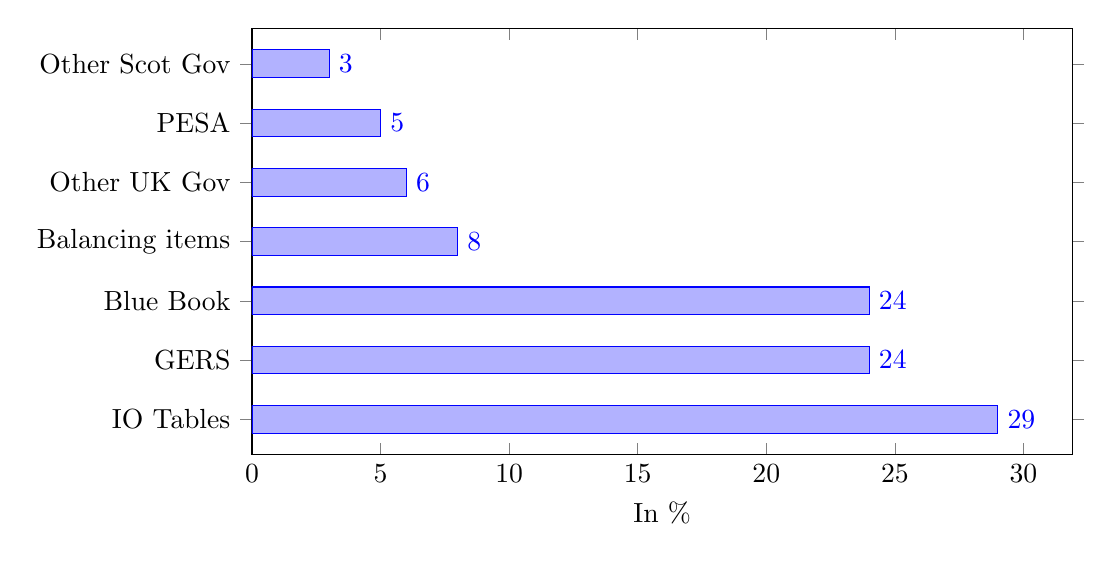
\begin{tikzpicture}
  \begin{axis}[xbar, xmajorgrids=false, xmin=0, width=12cm, height=7.0cm, enlarge y limits=0.1, xlabel={In $\%$},symbolic y coords={IO Tables,GERS,Blue Book,Balancing items,Other UK Gov,PESA,Other Scot Gov},ytick=data,nodes near coords, nodes near coords align={horizontal},] \addplot coordinates {(29,IO Tables) (24,GERS) (24,Blue Book) (8,Balancing items) (6,Other UK Gov) (5,PESA) (3,Other Scot Gov) }; \end{axis}
  \end{tikzpicture} \end{center} \end{scriptsize} \label{fig:2.4.1} \end{figure}

\bigskip

Figure \ref{fig:2.4.1} shows that the largest source of data for the IncExp Accounts originates from the 2009 IO Tables for Scotland with 29\% \cite{ScotGov2013a}. The other two major data sources are depicted as GERS with 24\% \cite{ScotGov2013b} and the ONS Blue Book, i.e. the UK National Accounts, with 24\% \cite{ONS2011c}. Figure \ref{fig:2.4.1} also highlights that the majority of data used in the compilation of the IncExp Accounts originates from Scottish data. Summing up the shares of 2009 IO Tables, GERS and other Scottish Government sources shows that approximately 56\% of data is of Scottish origin. The total amount based on UK data sources is calculated at 35\%, which is the sum of the shares of the ONS Blue Book, Other UK Government and Public Expenditure Statistical Analysis (PESA) \cite{HMTR2012}\footnote{The shares are 24\%, 6\% and 5\% respectively.}. Figure \ref{fig:2.4.1}  shows furthermore that Balancing Items account for 8\% of total individual entries in the Accounts. Essentially, these are elements which are determined through the requirement that the expenditures and receipts in each account must balance. Note that a full discussion on Balancing Items can be found in Section \ref{sec:2.4.3}. Data consistency of the IncExp Accounts is ensured since only a small number of data-consistent official sources are used (see Figure \ref{fig:2.4.1}).

\bigskip

\subsubsection{Data Sources}

The largest data source for the calculation of the IncExp Accounts are the 2009 IxI (IO) Tables. The 2009 Tables are the latest IO Tables released by the Scottish Government at the time of this publication and henceforth they determine the year for which the Scottish SAM is built. The IO Tables furthermore determine the accounting period of the IncExp Accounts and the SAM, which is the calendar year format. The Scottish IO Tables and thus the Scottish SAM represent the Scottish onshore economy only, and do not include revenue from North Sea oil and gas operations. It has to be noted that other data sources used in the compilation of the IncExp Accounts, for example the ONS Blue Book \cite{ONS2011c}, include revenue from North Sea operations. This directly affects the Scottish GDP as a share of total UK GDP (see Equation \ref{eq:2.5.80}), which is derived by figures from the IO Tables and the ONS Blue Book respectively \cite{ScotGov2013a, ONS2011c}. The Scottish GDP is underestimated in this instance in relation to the UK GDP figure. 

\bigskip

The second largest source for data used in the IncExp Accounts is Government Expenditure and Revenue Scotland (GERS), which is an annual publication by the Scottish Government. GERS uses both UK and Scottish Government finance statistics in order to capture all public sector expenditures and receipts in Scotland. This source provides, inter alia, household and corporate tax payments as well as total public spending control totals for the IncExp Accounts\footnote{This corresponds to (Cell 43)}. The data in GERS are presented in financial year format and have to be transformed to the calendar year format (as discussed above) for the IncExp Accounts \cite{ScotGov2013b}.

\bigskip

The third largest data source used here is the ONS Blue Book, i.e. the UK National Accounts, which is an annual UK National Statistics Publication. The Blue Book is constructed using governmental financial statistics, both from the UK- as well as international government sources. It provides a detailed sectoral breakdown of the UK economy as well as its economic activities with the rest of the world (ROW). The Blue Book data are used for a wide variety of entries in the Accounts, for example, public and private dividend payments to household. The data is in the calendar year format and do not require transformation \cite{ONS2011c}.

\bigskip

The fourth largest single source for the IncExp Accounts is the data from the annual HM Treasury Public Expenditure Statistical Analysis (PESA) publication. Here Local and Central Government spending is detailed, including the budgets of UK government department. PESA is a major source for the GERS publication by the Scottish Government \cite{ScotGov2013b}. The data used in the IncExp Accounts originating from PESA are public sector identifiable, non-identifiable and total spending. The data are presented in financial year format and have to be transformed to the calendar year format for the IncExp Accounts \cite{HMTR2012}.

\bigskip

Finally, there are other UK and Scottish Government sources. These include, for example, figures used for the derivation of Scottish households as a share of total UK households (see Equation \ref{eq:2.5.82}) \cite{ScotGov2012c, ONS2012}.

\bigskip

\subsubsection{Shares}

As mentioned above, several shares are used in order to transform UK data for the Scottish IncExp Accounts. These shares are essential as some data are only available on the UK level. For example, the Total Managed Public Sector Expenditure in PESA \cite{HMTR2012}, which is used to estimate the total public expenditure in Scotland\footnote{This is the Total Government Expenditure Balancing Total (Cell 43) in the IncExp Accounts}.

\bigskip

The various shares are used throughout the derivations of the individual cells of the IncExp Accounts. The three shares used for the majority of UK data transformation are given below. These are the GDP share at 8.22\% (see Equation \ref{eq:2.5.80}), the Population share at 8.41\% (see Equation \ref{eq:2.5.81}) and the Households share at 9\% (see Equation \ref{eq:2.5.82}). Other shares, such as the Scottish share of Total UK Other Value Added at 8.31\% (see Equation \ref{eq:2.5.85}) are also used in the calculations (see Section \ref{sec:2.5} for further details). These shares are all close in value. However, theoretical considerations favour different shares for specific UK data as outlined below.

\bigskip

First, the GDP share is applied when UK data is transformed for the Scottish jurisdiction. For example, Governmental and Corporate transfers payments \cite{ONS2011c} are multiplied by the GDP share following the framework set out by \shortciteA{Hermannsson2010a}. Second, the Population share is used for public sector spending, which is allocated to the different jurisdictions within the UK through size estimates of the relevant region. This is in line with the methodology applied in GERS \cite{ScotGov2013b} for transforming PESA \cite{HMTR2012} data for Scotland. Third, the Household share is applied to transform UK Dividend Payments to a Scottish figure, which follows UK calculations in transforming total dividend payments to the household level \cite{ONS2011c}.

\bigskip

The majority of data used in the IncExp Accounts is derived from Scottish sources as outlined above. Nevertheless, many statistics are only available on the UK level and the Scottish figure has to be inferred as a share of that. Increasing the volume of entries calculated from direct Scottish data would result in more accurate IncExp Accounts.

\newpage

%%%%%%%%%%%%%%%%%%%%%%%%%%%%%%%%%%%%%%%%%%%%%%%%%%%%%%%%%%
%SUBSECTION
%%%%%%%%%%%%%%%%%%%%%%%%%%%%%%%%%%%%%%%%%%%%%%%%%%%%%%%%%%
\subsection{Layout}
\label{sec:2.4.2}

\bigskip

The IncExp Accounts (see Table \ref{tab:2.4.1}) are divided into five sectors (Households, Corporations, Government, Capital and External) as well as the Scottish Trade and External balance with both the RUK and the ROW. Each of those sectors is divided further into an income and an expenditure section (left-hand side and right-hand side respectively), hence the name for these Accounts.

\bigskip

Each numerical entry in the IncExp Accounts (see Table \ref{tab:2.4.1}) is referred to as a cell and is identified for convenience through the number code given to each entry. For example, (Cell 19) refers to the Profit Income (OVA) of the Corporations' Income Account.

\bigskip

Every account has a Total Income and a Total Expenditure figure, which is a summation of the entries in each section (highlighted in bold). The total expenditure and the total income for each of the main transactors as well as for the Capital account are equal to each other. This is essential for the balancing of the SAM and is discussed in more detail in Section \ref{sec:2.4.3} under ``Balancing Items''. In addition to the totals derived by summing up the individual entries in each of the main transactors' accounts, the Household and Government sector have additional Control Totals from external sources. For the Household Sector this is (Cell 1), which is the Total Household Income from the GDHI figures \cite{ONS2011b}. For the Government sector the Control Total is (Cell 43), which is the total public sector expenditure in Scotland derived from GERS and the PESA accounts \cite{ScotGov2013b, HMTR2012}.

\bigskip

The main transactors (Households, Corporations and Government) have a similar cell breakdown. The largest share of entries in these accounts are Income from- and payments to the other main transactors as well as flow of funds to and from the External account. Note that due to the accounting identity used in the IncExp Accounts, the receipt that, for example, sector A receives form sector B is equal to the payment made by sector B to sector A. This is discussed in more detail in Section \ref{sec:2.4.3} under ``Corresponding Figures''. The External payments are comprised of goods \& services payments and receipts to and from Scotland to both RUK and ROW. Additionally, they show the sums of the transfers to and from RUK and ROW by the main transactors. For example, (Cell 53) are the Transfers that Scotland pays to RUK, which is the sum of (Cells 14, 27 and 41). Furthermore, all main transactors have a Profit Income (OVA) entry and a Payments to Capital\footnote{These are equal to savings made by the individual sector and the Payments to Capital of each sector are used to derive the Capital account.} entry on the Income and on the Expenditure side, respectively.


% % % % % % % % % % % % % % % % % % % % % % % % % % % % % % % % %
% % % % % % THE INCOME AND EXPENDITURE ACCOUNTS TABLE % % % % % %
% % % % % % % % % % % % % % % % % % % % % % % % % % % % % % % % %


\begin{table}[H] \caption{Income-Expenditure Accounts for Scotland (in \textsterling million)}
\bigskip \begin{scriptsize} \begin{centering} \begin{spacing}{1.2}
    \begin{tabular}{lrllrl}
          \toprule
    \textbf{HOUSEHOLDS} \bigstrut\\
   \hline  
\bigstrut[t]    1. \textbf{Income} & \textbf{107877} & & 10. \textbf{Expenditure} & \textbf{107877} & \\
    2. Income from Employment & 63561  &   & 11. IO Expenditure & 74669 & \\
    3. Profit Income (OVA) & 5289 & & 12. Payments to Corporations & 6401 &* \\
    4. Income from Corporations & 15103 & & 13. Payments to Government & 21379 & \\
    5. Income from Government & 19835 & & 14. Transfers to RUK & 238 & \\
    6. Transfers from RUK & 1853 & & 15. Transfers to ROW & 119 & \\
    7. Transfers from ROW & 2237 & & 16. Payments to Capital (Savings) & 5070 &\\
    8. Mixed and Proport. Income Unalloc. & 867 &* & &\\
    9. \textbf{Total Household Income} & \textbf{107877} & & 17. \textbf{Total Expenditure} & \textbf{107877} &**\\
    \hline
\bigstrut[t]    \textbf{CORPORATIONS} \bigstrut\\
    \hline
\bigstrut[t] 18. \textbf{Income} & \textbf{53507}  &   & 24. \textbf{Expenditure} & \textbf{53507} & \\
       19. Profit Income (OVA) & 29456 & & 25. Payments to Households & 15103 &** \\
       20. Income from Households & 6401 &** & 26. Payments to Government & 5248 & \\
       21. Income from Government & 5722 &** & 27. Transfers to RUK & 3768 & \\
       22. Income from RUK & 5964 & & 28. Transfers to ROW & 4560 & \\
       23. Income from ROW & 5964 & & 29. Payments to Capital (Savings) & 24828 &* \\
    \hline
    \textbf{GOVERNMENT} \bigstrut\\
    \hline
\bigstrut[t]       30. \textbf{Income} & \textbf{63530}  &   & 37. \textbf{Expenditure} & \textbf{63530} & \\
       31. Profit Income (OVA) & 3697 & & 38. IO Expenditure & 29486 & \\
       32. Net Commodity Taxes & 13165 & & 39. Payments to Corporations & 5722 &* \\
       33. Income from Households & 21379 &** & 40. Payments to Households & 19835 &** \\
       34. Income from Corporations & 5248 &** & 41. Transfers to RUK & 8368 & \\
       35. Income from RUK & 20041 &* & 42. Payments to Capital (Savings) & 119 & \\
       36. \textbf{Total Gov Inc Balancing Total} & \textbf{63530} &** & 43. \textbf{Total Gov Exp Balancing Total} & \textbf{63530} &  \\
    \hline
    \textbf{CAPITAL} \bigstrut\\
    \hline
\bigstrut[t]       44. \textbf{Income} & \textbf{19930}  &   & 49. \textbf{Expenditure} & \textbf{19930} & \\
       45. Households & 5070 &** & 50. IO Expenditure & 19930 &  \\
       46. Corporations & 24828 &** &  \\
       47. Government & 119 &** &  \\
       48. RUK/ROW & -10087 &** &  \\
    \hline
    \textbf{EXTERNAL} \bigstrut\\
    \hline
\bigstrut[t]  51. RUK Income from Scotland & 67133  &   & 58. RUK Expenditure in Scotland & 70597 & \\
       52. Goods \& Services from RUK & 54759 & & 59. Goods \& Services to RUK & 42739 & \\
       53. Transfers to RUK & 12374 & & 60. Transfers from RUK & 27858 & \\
       54. ROW Income from Scotland & 23676 & & 61. ROW Expenditure in Scotland & 27378 & \\
       55. Goods \& Services from ROW & 18997 & & 62. Goods \& Services to ROW & 19178 & \\
       56. Transfers to ROW & 4679 & & 63. Transfers from ROW & 8201 & \\
       & & & 64. Tourist Expenditure in Scotland & 2921 & \\
       57. \textbf{Total Income} & \textbf{90808} & & 65. \textbf{Total Expenditure} & \textbf{100896} &  \\  
        & & & 66. Surplus/Deficit &-10087 & \\  
    \hline
    \textbf{G\&S TRADE BALANCE} & & & \textbf{TOTAL BALANCE OF PAYMENTS} \bigstrut\\
    \hline
       67. RUK & -12020 & & 69. RUK & 5217 &  \\
       68. ROW & 181 & & 70. ROW & 4871 & \\
       & & & 71. Total Balance of Payments & 10087 & \\  
    \hline    
    \textbf{EXTERNAL BALANCE} \bigstrut\\
    \hline
\bigstrut[t]   72. Income from Employment & -3464 & & & & \\
       73. Profit Income (OVA) & -3703 & & & &  \\
       74. Income from Corporations & -2921 & & & & \\
       75. Income from Government & -10087 & & & & \\
    \bottomrule  \bigstrut[b]\\
\qquad \qquad \qquad Balancing Item: *   & & & Row Entries (Element determines Column)  \\
\qquad \qquad \qquad Corresponding Figure: ** & & & Row Entries (Element determines Column)  \bigstrut\\      
   \end{tabular}%  
\bigskip \begin{flushright}\end{flushright} \label{tab:2.4.1}
\end{spacing} \end{centering}  \end{scriptsize} \end{table}



%%%%%%%%%%%%%%%%%%%%%%%%%%%%%%%%%%%%%%%%%%%%%%%%%%%%%%%%%%
%SUBSECTION
%%%%%%%%%%%%%%%%%%%%%%%%%%%%%%%%%%%%%%%%%%%%%%%%%%%%%%%%%%
\subsection{Calculation Overview and Internal Balancing}
\label{sec:2.4.3}

\bigskip

The structure used for compiling the IncExp Accounts follows a framework set out by \shortciteA{Hermannsson2010a}, which also used data from both the Scottish IO Tables as well as other external sources. As stated above, the largest share of data entries originates from the 2009 IO Tables for Scotland \cite{ScotGov2013a}. The entries in the IncExp Accounts, which are calculated solely with data from the IO Tables, do not have to be transformed in order to fit these into the SAM framework. For example, (Cell 11) and (Cell 38) are summations of several IO entries.

\bigskip

Linking together the IncExp Accounts (see Table \ref{tab:2.4.1}) and the IxI Table (see Table \ref{tab:2.3.1}) is described in the following by the means of using the Government account as an example. Table \ref{tab:2.4.2} depicts the Government account in an aggregate 2009 Scottish SAM. In the parenthesis of the SAM figures the location within the IncExpAccounts or IO table is detailed. For example, the \textsterling29,486m Government expenditures on Activities stem from the IO table (Table \ref{tab:2.3.1}). The \textsterling119m of Government expenditures on Capital stem from the IncExp Account and can be found in (Cell 49) in Table \ref{tab:2.4.1}.

\bigskip

Due to the aggregation of the SAM (Table \ref{tab:2.4.2}) it is necessary to combine IO and IncExp data for several entries. For example, the \textsterling27,947m Government income from Households is the sum of (Cell 33) `Payments to Households to Government' and the IO entry `Taxes on Expenditure'. Thus, it mus be stressed again, that this aggregation is for illustration purposes only and that the fully disaggregated table should be consulted when evaluating the figures contained within the SAM.

\bigskip

  \begin{table}[H] \caption{Linking together IO tables and the IncExp Accounts, 2009 basic prices (\textsterling million)}
  \bigskip \begin{scriptsize} \begin{centering} \begin{doublespacing}
  \begin{tabular}{lrrrrrrrrr}
  \toprule
  & \begin{sideways}1. Activities \end{sideways} &
  \begin{sideways}2. Labour \end{sideways} &
  \begin{sideways}3. Capital \end{sideways} &
  \begin{sideways}4. Other Value Added \end{sideways} &
  \begin{sideways}5. Households \end{sideways} &
  \begin{sideways}6. Corporations \end{sideways} &
  \begin{sideways}7. Government \end{sideways} &
  \begin{sideways}8. RUK \end{sideways} &
  \begin{sideways}9. ROW \end{sideways} \bigstrut[b]\\
  \hline
  Gov Expenditures  & 29,486  &  \: \: \: - &  119  & - & 19,835  & 5,722  & 13,165  & 8,368  &  - \\
  (Column in SAM) &  (IO)  &  - &  (Cell 49)  & - &  (Cell 40)  &  (Cell 39)  &  (Cell 32)  &  (Cell 41)  &  - \\
  & & & & & & & & &  \\
  Gov receipts & 4,779  &  - & 1,495  & 3,697  & 27,947  & 5,248  & 13,165  & 20,234  &  129  \\
  (Row in SAM) & (IO) &  - & (IO) & (Cell 31) & (Cell 33+IO) & (Cell 34) & (Cell 32) & (Cell 35+IO) & (IO)
  \bigstrut[t]\\
  \bottomrule \end{tabular}%
  \bigskip \begin{flushright} Note: The location of the figures in the IncExp Accounts and the IO Tables are detailed in the parenthesis.\end{flushright} \label{tab:2.4.2}
  \end{doublespacing} \end{centering} \end{scriptsize} \end{table}

\bigskip

Additional to the IO Tables and the other data sources discussed in the Section \ref{sec:2.4.1}, the IncExp Accounts contain internally derived cells. These are notated with a single star (*) for Balancing Items and with two stars (**) for Corresponding Figures (see Table \ref{tab:2.4.1}).

\bigskip

\subsubsection{Balancing Items}

Balancing Items are used to balance the Total Income and the Total Expenditure of the main transactors. The method used for allocating Balancing items to the various accounts is as follows. The Household and Government accounts have control totals and in order to balance total income with total expenditure for these accounts, manual balancing is needed. Thus, there is a Balancing Item on the income and on the expenditure side for each one of these accounts. The Corporate Account does not have control totals, however. Within the Corporate account, the income entries are more robust than the expenditure ones. Therefore we impose the balancing on the latter. Generally, Balancing Items are imposed on those cells, for which data availability or quality is least robust.

\bigskip

Balancing Items are calculated by summing up all figures of one sector on the relevant account side (apart from the cell used as a Balancing Item) and deducting the Total figure by that calculated sum. For example, Corporations' Payments to Capital (Cell 29) is calculated through deducting the sum of (Cell 25) to (Cell 28) from the total Expenditure (Cell 24).

\bigskip

\subsubsection{Corresponding Figures}

As outlined in the previous section, based on the accounting identity used for the IncExp Accounts, the income that sector A receives from sector B is equal to the payment that sector B makes to sector A. Thus there is a correspondence between payments of the main transactors to each other in the IncExp Accounts. For example, the Income from Corporations received by the Government (Cell 34) is equal to the Payments to Government made by Corporations (Cell 26).

\bigskip

It must be noted that the sequence of the Accounts determines the use and presence of Corresponding Figures. The sequence of the IncExp Accounts is set out to be: 1.Households, 2.Corporations, 3.Government, 4.Capital to last 5.External. Corresponding Figures between the main transactors occur only in the accounts that follow the Household account. The Household account's Total Expenditure (Cell 17), is an `account internal Corresponding Figure' referencing Total Household Income (Cell 9) and thus not an entry corresponding to another main transactor.

\bigskip

The use of Corresponding Figures is only then problematic when it corresponds to a cell that is calculated as a Balancing Item. For example, all income entries for the Capital account are Corresponding Figures, as these are equal to the Payments to Capital entries by each of the Primary Sectors (Cells 16, 29 \& 42) as well as the net External balance (Cell 66). The entry that could cause a `compounded error' due to reusing a Balancing Item, here, is Capital Income from the Corporate account (Cell 46) which corresponds to the Corporations' Payments to Capital (Cell 29), which is a Balancing Item.

\bigskip

Table \ref{tab:2.4.3} provides details of the cells of the IncExp Accounts, which highlights, inter alia, whether cells are derived through external sources or through internal calculation. Cells noted as ``Regular'' are simply cells in the IncExp Accounts, which are marked as neither Balancing Items nor Corresponding Figures (see Table \ref{tab:2.4.1}). The slight majority of the ``Regular '' cells is derived through internal calculations (with 29 internally calculated cells versus 28 externally calculated cells). For example, Total Household Income (Cell 9), which is the total of all cells in the Households' income account, is internally calculated. The cells noted as being externally calculated are those, which were derived through figures external to the IncExp Accounts. For instance, the Households' Payments to Government (Cell 13) is calculated through figures taken solely from GERS \cite{ScotGov2013b}.

\bigskip

The second row of Table \ref{tab:2.4.3} shows that there are a total of 5 Balancing Items in the IncExp Accounts. These are all internally derived, following the method outlined above. Note that three of those Balancing Items are used within the Accounts as Corresponding Figures and could thereby be the source of a `compounding error'\footnote{Where Corresponding Figures refer to a cell that is calculated as a Balancing Item, it is marked as such in the detailed breakdown in Section \ref{sec:2.5}}.

\bigskip

Cells noted as Corresponding Figures in the IncExp Accounts are detailed in row three of Table \ref{tab:2.4.3}. Four of these cells are denoted as being derived from internally calculated cells. Three of those are the above-mentioned Balancing Items, which are also used as Corresponding Figures. The fourth internally derived Corresponding Figure is the Household sector's Total Expenditure (Cell 17). This cell is equal to Total Household Income (Cell 9), which is a summation of all income of the Household sector. All other Corresponding Figures are equal to externally calculated cells. For example, Government's Payments to Households (Cell 40) is equal to Household's Income from Government (Cell 5), which are derived through figures from both both GERS and the ONS Blue Book \cite{ScottishGovernment2013a, ONS2011c}. Note that although thirteen cells are identified as Corresponding Figures in the Accounts, in effect 26 cells have corresponding entries to other cells. If the ordering of the Accounts were different, for example the Household account would follow the Government account, then Household's Income from Government (Cell 5) would be a Corresponding Figure of Government's Payments to Households (Cell 40). Thus (Cell 5) would be noted as a Corresponding Figure and (Cell 40) would not be.

\bigskip

Table \ref{tab:2.4.3} highlights that in total 38 cells are calculated through external sources, whilst 37 cells in the Accounts are derived through internal calculation. The entries of the main transactors are mainly obtained through external sources whilst the majority of entries from the Capital account and below (see Table \ref{tab:2.4.1}) are derived through internal calculations.

\bigskip
\begin{centering}
  \begin{table}[H]
\centering
  \caption{Income and Expenditure Cell Details}
  \bigskip \begin{scriptsize}  \begin{doublespacing}
  \begin{tabular}{lccc}
  \toprule
  & Internal
  & External
  & Total  \bigstrut[b]\\
  \hline
  1. Regular &  29  & 28  &  57   \\
  2. Balancing Item &  5  &  -  &  5   \\
  3. Corresp. Figure &  4  &  9  &  13    \bigstrut[b]\\
  \hline
  Total &  38  &  37  &  75    \bigstrut[t]\\
      \bottomrule \end{tabular}%
      \bigskip  \label{tab:2.4.3}
      \end{doublespacing}  \end{scriptsize} \end{table}
      \end{centering}
\bigskip

Concerning future work on the IncExp Accounts, the reliance on Balancing Items could be looked into further. As Figure \ref{fig:2.4.1} shows, these cells account for 8\% of the total individual entries for the IncExp Accounts. Currently, the cells for which we have the least robust data are chosen in order to balance the accounts of the main transactors. If robust estimates for these entries could also be obtained, then the balancing of the account could be distributed across a number of cells in an account. However, determining the balancing share of each entry might prove difficult and could result in a number of robust estimates to be skewed.

\newpage


%%%%%%%%%%%%%%%%%%%%%%%%%%%%%%%%%%%%%%%%%%%%%%%%%%%%%%%%%%
%SECTION
%%%%%%%%%%%%%%%%%%%%%%%%%%%%%%%%%%%%%%%%%%%%%%%%%%%%%%%%%%
\newpage
\section{Income and Expenditure Accounts - Method}
\label{sec:2.5}

\bigskip
\begin{center}
\textbf{\LARGE Households}
\end{center}

\begin{enumerate}


\item \textbf {Income}

\bigskip

The Household income entry is derived from the latest revised figures of Scottish Gross Disposable Household Income (GDHI) for 2009 at NUTS2 level \cite{ONS2013a}. This figure is then used within the IncExp Accounts as a control total.

\bigskip

\begin{equation}
\begin{split}
\text{Total Income} =  \\ \\
\text{Operating surplus and Mixed income}\\
+\text{Compensation of employees}\\
+\text{( Property income, received - Property income, paid)}\\
+\text{Imputed social contributions and Social benefits}\\
+\text{( Other current transfers, received - Other current transfers, paid)}\\
\end{split} \label{eq:2.5.1}
\end{equation}

\begin{equation} \nonumber
107877 = 9437 + 64645 + (8485 - 551) + 23559 + (5102 - 2800)
\end{equation}\\


\item \textbf {Income from Employment}

This is the ``Compensation of employees'' \text{||} ``Total intermediate demand'' from one source, the IO Tables and the data from this source are taken to be fixed\footnote{References from the IO Tables are identified by first the column and then the row. In order to distinguish these the convention || is used between the name of the IO column and the name of the IO row.}. The data of the IO Tables is presented in the calendar year format and thus no adjustment is needed.  The ``Compensation of employees'' in the IO Tables does include wage payments as well as non-wage labour costs, such as NI contributions \cite{ScottishGovernment2013a}.

\begin{equation}
\begin{split}
\text{Income from Employment} =  \\ \\
(\text{Compensation of Employees}\|\text{Total Intermediate Demand})
\end{split} \label{eq:2.5.2}
\end{equation}

\begin{equation} \nonumber
63561 = 63561
\end{equation}\\

\newpage

\item \textbf {Profit Income (OVA)}

\bigskip

This entry requires that the Gross Operating Surplus for Scotland is identified. Yet, these data are only available as an aggregate comprising of Operating surplus and Mixed Income. Therefore, the `Operating surplus and Mixed income' figure is disaggregated to identify the Gross Operating Surplus and Mixed Income component separately. This is estimated by using shares derived from 1999 GDHI data which is the last data-set to report these figures individually. There are no alternative datasets available that would allow for a better estimation of Scottish Gross Operating Surplus for 2009.

\bigskip

GDHI data for 1999 is obtained from \shortciteA{Hermannsson2010a} and the shares of Gross Operating Surplus and Mixed Income are calculated. Gross Operating Surplus comprises of 56 percent and Gross Mixed Income comprises of 44 percent of total Operating and Mixed surplus and Mixed Income in 1999. These shares are used to disaggregate the aggregate 2009 figure. This process yields the required Gross Operating Surplus estimate for Scotland of \textsterling5,289m. Thus, 2009 data (the control total) is disaggregate by using 1999 shares to yield the necessary Gross Operating Surplus which is used as Household Profit Income in the IncExp Accounts \cite{ONS2011b}.

\begin{equation}
\begin{split}
\text{Profit Income} = \\ \\
\text{Operating surplus and Mixed income} \\
* \text{1999 Share of Gross operating surplus}
\end{split} \label{eq:2.5.3}
\end{equation}

\begin{equation} \nonumber
5289 = 9437 * 0.56\%
\end{equation}\\


\newpage

\item \textbf {Income from Corporations}

The income households receive from corporations is the sum of Capital Gains, then any non-wage payments received and lastly from mixed and proportionate income\footnote{This is a Balancing Item.} calculated in the Income Accounts for Households.

\bigskip

First, deriving the Capital Gains Tax receipts from GERS and dividing them by the fixed  Capital Gains Tax Rate for 2008-10 (at 18\%), gives an estimate of the actual monetary value of the capital gain received by Scottish households for 2009 at \textsterling1,478m\cite{ScotGov2013b,HMRC2013}.\\
Second, the non-wage income received by households from corporations is calculated. This comprises multiplying the Scottish GDP share (see Equation \ref{eq:2.5.80}) by the total of ``UK Private Dividends'' paid out by private non-financial corporations in the UK. The calculated figure is then multiplied by the individual's share of total equity\footnote{This share is an average for the years 2008 and 2010, since a figure for 2009 is not available. This share is based on a UK-wide total equity share of individual's.}, which gives an estimate of the dividend payments by non-financial corporations received by Scottish households at at \textsterling765m. This is then used to distinguish the dividend payments received by private shareholders versus, for example, funds \cite{ONS2011c}. Further, this part of the income figure is derived by adding an estimate of the ``Total Private Pensions'' \footnote{No estimate for Scottish Private Pension payments for 2009 could be obtained. This figure here is using the share of Scottish private pensions against Social Security payments received by households. This share is obtained from a 2006 Scottish SAM \cite{Hermannsson2010a} and multiplied by the 2009 Social Security payments for Scotland.} received by Scottish households at \textsterling9,691m as well as household's ``Net Other Income'' from the GDHI at at \textsterling2,302m to the non-wage income received by households from corporations\cite{ONS2012}.\\
Third, Households' Mixed and Proportionate Income Unallocated (Cell 8) at at \textsterling867m is added in order to balance this part of the Accounts.  


\begin{equation}
\begin{split}
\text{Income from Corporations} =  \\ \\
\text{Household Income from Capital Gains}\\
+\text{Household Income from Corporations}\\
+\text{Mixed and Proportionate Income Unallocated}_\text{IncExp}\\
\end{split} \label{eq:2.5.4}
\end{equation}

\begin{equation} \nonumber
15103 = 12758+1478+867
\end{equation}

\begin{center}
\line(1,0){250}
\end{center}


\textit{where}

\begin{equation}
\begin{split}
\text{Household Income from Capital Gains} = \\
(1/4 *\text{Households' Capital Gains Tax Payments}_\text{08-09}\\
+ 3/4 *\text{Households' Capital Gains Tax Payments}_\text{09-10})\\
\div \text{Capital Gains Tax Rate}
\end{split} \label{eq:2.5.5}
\end{equation}

\begin{equation} \nonumber
1478 = (1/4*572+3/4*164)\div 18\%
\end{equation}

\begin{center}
\line(1,0){250}
\end{center}

\newpage


\begin{equation}
\begin{split}
\text{Total Household Income from Corporations} = \\
(\text{Scottish GDP Share}*\text{Individual Share of Total Equity}\\
*\text{Total UK Private Dividend Payments})\\
+ \text{Total Private Pension}+ \text{Net Other Income}
\end{split} \label{eq:2.5.6}
\end{equation}

\begin{equation} \nonumber
12758 = 8.22\% * (\frac{10.2\%+11.5\%}{2}) * 85816+9691+2302
\end{equation}

\begin{center}
\line(1,0){250}
\end{center}


\begin{equation}
\begin{split}
\text{Mixed and Proportionate Income Unallocated} = \\
(\text{Total Household Income}_\text{GDHI}-\text{Total Household Income}_\text{IncExp})\\
\end{split} \label{eq:2.5.7}
\end{equation}

\begin{equation} \nonumber
867 = 107877-107010
\end{equation}\\

\item \textbf {Income from Government}

This figure comprises the annualised ``Social Protection Payments'' to Scottish households \cite{ScotGov2013b} and the ``Public Dividend Payments'' received by Scottish households \cite{ONS2011c}. The latter is calculated in accordance with the methodology outlined above for ``Private Dividend Payments''. The dividend payments are sourced from non-financial corporations, Central Government and Local Government accounts and are multiplied by the Scottish GDP share as well as the average individual`s share of total equity and further multiplied by the UK Public Dividend payments.  

\begin{equation}
\begin{split}
\text{Income from Government} =  \\ \\
(1/4*\text{Total Social Protection}_\text{08-09}\\
+3/4*\text{Total Social Protection}_\text{09-10})\\
+\text{Scottish GDP Share} \\
*(\text{UK Public Dividends}_\text{Non-Financial Corporations}\\
+\text{UK Public Dividends}_\text{Central Government}\\
+\text{UK Public Dividends}_\text{Local Government})\\
*((\text{Individual's Share of Total Equity}_\text{2008}\\
+\text{Individual's Share of Total Equity}_\text{2010})\div 2)
\end{split} \label{eq:2.5.8}
\end{equation}


\begin{equation} \nonumber
\begin{split}
19835 = (1/4*18653+3/4*20193)\\
+(8.22\%*(25+2214+772)*((10.2\%+11.5\%)\div 2))
\end{split}
\end{equation}\\


\item \textbf {Transfers from RUK}

These transfers are calculated by, first, deriving the total figure of dividends paid to Scottish households. This figure is calculated by using the share of Scottish Households over total UK Households (see Equation \ref{eq:2.5.82})\footnote{the Household share is used here, since these are dividends paid to Scottish households specifically.} and multiplying it by ``Total RUK Dividends'' paid to UK households \cite{ONS2011c}. The latter figure is based on the average individual's share of total equity multiplied by the difference between Total UK- and Total Scottish- private dividends in order to obtain the RUK dividend payments to Households in Scotland \cite{ONS2011a,ONS2011b}.
Second, the difference of the ``Compensation of Employees'' according to the GDHI estimates and the actual figure of income from employment (Cell 2) is derived. The figures obtained from the first calculation and the second one are then summed up.


\begin{equation}
\begin{split}
\text{Transfers from RUK} =  \\ \\
\text{Total RUK Dividends to Scottish Households}\\
+(\text{Compensation of Employees}_\text{GDHI}\\
-\text{Income from Employment}_\text{IncExp})
\end{split} \label{eq:2.5.9}
\end{equation}

\begin{equation} \nonumber
1853= 767+(64645-63561)
\end{equation}\\

\begin{center}
\line(1,0){250}
\end{center}

\textit{where}

\begin{equation}
\begin{split}
\text{Total RUK Dividends to Scottish Households}=\\
\text{Scottish Household Share}*\text{Total RUK Dividends to Households}
\end{split} \label{eq:2.5.10}
\end{equation}

\begin{equation}\nonumber
767=9\%*8546
\end{equation}

\newpage

\item \textbf {Transfers from ROW}

This figure is calculated in two parts. First, the UK employment income from ROW \cite{ONS2011c} is calculated with the Scottish share of Total Corporate OVA (see Equation \ref{eq:2.5.85}). Using the Total Corporate OVA share for Scotland results in the most accurate estimate for this figure, since the Transfers from ROW are based on corporate flows of funds. Second, the amount of ``UK Property and Entrepreneurial Income'' is multiplied by the Scottish share of UK GDP (see Equation \ref{eq:2.5.80}) and by the Scottish household share of OVA for UK property and entrepreneurial income \cite{ScotGov2013a,ScotGov2013b}.

\begin{equation}
\begin{split}
\text{Transfers from ROW} =  \\ \\
(\text{Scottish Share of UK Total OVA}*\\
\text{UK Employment Income from ROW})\\
+(\text{Scottish Household OVA}*\text{Scottish GDP Share of UK}\\
*\text{UK Property and Entrepreneurial Income})
\end{split} \label{eq:2.5.11}
\end{equation}


\begin{equation} \nonumber
2237 = (143588.31\%)+(169313*15\%*8.22\%)
\end{equation}\\


\item \textbf {Mixed and Proportionate Income Unallocated}

Balancing Item: equal to the difference between the control total for Households' Income (Cell1) and Total Household Income (Cell 9) \cite{ONS2012}.

\begin{equation}
\begin{split}
\text{Income Unallocated} =  \\ \\
\text{Income}^\text{Households}_\text{IncExp}\\
-\text{Income from Employment}^\text{Households}_\text{IncExp}
\end{split} \label{eq:2.5.12}
\end{equation}


\begin{equation} \nonumber
867 = 107877-107010
\end{equation}\\

\newpage


\item \textbf {Total Household Income}

Totals Figure: this figure is the sum of all of the above entries for this account, excluding the total household income figure obtained from the GDHI (sum of cells 2 to 8).

\begin{equation}
\begin{split}
\text{Total Household Income} =  \\ \\
(\text{Income from Employment}^\text{Households}_\text{IncExp}\\
+\text{Profit Income (OVA)}^\text{Households}_\text{IncExp}\\
+\text{Income from Corporations}^\text{Households}_\text{IncExp}\\
+\text{Income from Government}^\text{Households}_\text{IncExp}\\
+\text{Transfers from RUK}^\text{Households}_\text{IncExp}\\
+\text{Transfers from ROW}^\text{Households}_\text{IncExp})
\end{split} \label{eq:2.5.13}
\end{equation}

\begin{equation} \nonumber
107877 = 63561+5289+15103+19835+1853+2237
\end{equation}\\


\item \textbf {Expenditure}

Totals Figure: Summation of figures below, from IO Expenditure to Payments to Capital (Cells 11 to 16).

\begin{equation}
\begin{split}
\text{Expenditure} =  \\ \\
\text{IO Expenditure}^\text{Households}_\text{IncExp}\\
+\text{Payments to Corporations}^\text{Households}_\text{IncExp}\\
+\text{Payments to Government}^\text{Households}_\text{IncExp}\\
+\text{Transfers to RUK}^\text{Households}_\text{IncExp}\\
+\text{Transfers to ROW}^\text{Households}_\text{IncExp}\\
+\text{Payments to Capital}^\text{Households}_\text{IncExp}
\end{split} \label{eq:2.5.14}
\end{equation}

\begin{equation} \nonumber
107877 = 74669+6401+21379+5070+238+119
\end{equation}\\

\newpage

\item \textbf {IO Expenditure}

This cell presents the consumption expenditure, including taxes paid on products, by both Households and ``Non-Profit Institutions Serving Households'' (NPISH). Examples for what NPISHs are include churches, sport clubs and political parties. These institutions are generally not mainly funded by governments and serve households either for free or for relative low cost \cite{Eurostat2013}. The IO Expenditure figure is calculated by using data solely from the IO Tables. This cell is constructed of  ``Total Intermediate Consumption at basic prices'' || ``Households' Final Consumption Expenditure'' plus ``Taxes less Subsidies on Products'' || ``Households Final Consumption Expenditure'' and ``Total Intermediate Consumption at basic prices'' || ``Non-Profit Institutions Serving Households' Final Consumption Expenditure'' plus ``Taxes less Subsidies on Products'' || ``Non-Profit Institutions Serving Households' Final Consumption Expenditure'' from the IO Tables \cite{ScotGov2013a}.

\begin{equation}
\begin{split}
\text{IO Expenditure} =  \\ \\
\text{Total Intermediate Consumption}\|\text{Final Consumption Expenditure}_\text{Households}\\
+\text{Taxes less Subsidies on Products}\|\text{Final Consumption Expenditure}_\text{Households}\\
+\text{Total Intermediate Consumption}\|\text{Final Consumption Expenditure}_\text{NPISH}\\
+\text{Taxes less Subsidies on Products}\|
\text{Final Consumption Expenditure}_\text{NPISH}
\end{split} \label{eq:2.5.15}
\end{equation}\\

\begin{equation} \nonumber
74669 = 65421+6568+2680+0
\end{equation}\\


\item \textbf {Payments to Corporations}

Balancing Item: Taking the Total Expenditure (Cell 17) and subtracting the sum of: IO Expenditure (Cell 11), Payments to Government (Cell 13), Transfers to RUK (Cell 14), Transfers to ROW (Cell 15), Payments to Capital (Cell 16) from it.

\begin{equation}
\begin{split}
\text{Payments to Corporations} =  \\ \\
\text{Total Expenditure}^\text{Households}_\text{IncExp}\\
-\text{IO Expenditure}^\text{Households}_\text{IncExp}\\
-\text{Payments to Government}^\text{Households}_\text{IncExp}\\
-\text{Transfers to RUK}^\text{Households}_\text{IncExp}\\
-\text{Transfers to ROW}^\text{Households}_\text{IncExp}\\
-\text{Payments to Capital}^\text{Households}_\text{IncExp}
\end{split} \label{eq:2.5.16}
\end{equation}

\begin{equation} \nonumber
6401 = 107877-74662-21379-238-119-5070
\end{equation}\\


\item \textbf {Payments to Government}

These are the taxes paid by Households to the Government. The source for these entries is GERS and therefore these figures have to be annualised according to the method outlined above. These taxes are: Income Tax, Capital Gains Tax, Inheritance Tax, Stamp Duties, Half Insurance Premium Tax, Council Tax and Social Security Contributions (NI) \cite{ScotGov2013b}. The figures are annualised as detailed in Section \ref{sec:2.4.1}.

\begin{equation}
\begin{split}
\text{Payments to Government} =  \\ \\
1/4*(\text{Income Tax}_\text{08-09}+\text{Capital Gains Tax}_\text{08-09}\\
+\text{Inheritance Tax}_\text{08-09}+\text{Stamp Duties}_\text{08-09}\\
+\text{Half Insurance Premium Tax}_\text{08-09}+\text{Council Tax}_\text{08-09}\\
+\text{Social Security Contributions}_\text{08-09})\\
+3/4*(\text{Income Tax}_\text{09-10}+\text{Capital Gains Tax}_\text{09-10}\\
+\text{Inheritance Tax}_\text{09-10}+\text{Stamp Duties}_\text{09-10}\\
+\text{Half Insurance Premium Tax}_\text{09-10}+\text{Council Tax}_\text{09-10}\\
+\text{Social Security Contributions}_\text{09-10})\\
\end{split} \label{eq:2.5.17}
\end{equation}

\begin{equation} \nonumber
\begin{split}
21379=(1/4*(10642+572+178+594+96+1960+7992))\\
+(3/4*(10364+164+146+516+95+1961+7915))
\end{split}
\end{equation}\\


\item \textbf {Transfers to RUK}

This figure is calculated using the same methodology as outlined for (Cell 15). It is assumed that the transfers paid to the RUK are twice as high as those paid to the ROW, and thus this cell is equal to (Cell 15) times two.

\begin{equation}
\begin{split}
\text{Transfers to RUK} =  \\ \\
\text{Transfers to ROW}^\text{Households}_\text{IncExp}*2
\end{split} \label{eq:2.5.18}
\end{equation}

\begin{equation} \nonumber
238 = 119*2
\end{equation}\\

\newpage

\item \textbf {Transfers to ROW}

This figure is comprised of, first, the amount of employee compensation that is paid to the ROW, i.e. the part that is deducted from GDP in order to arrive at GNP figures. Then it is multiplied by the share of Scottish OVA of Corporate Income (see Equation \ref{eq:2.5.85}) \cite{ONS2011c}.

\begin{equation}
\begin{split}
\text{Transfers to ROW} =  \\ \\
\text{UK Payments to ROW}*\text{Scottish Corporate Income OVA}
\end{split} \label{eq:2.5.19}
\end{equation}

\begin{equation} \nonumber
119 = 1435*8.31\%
\end{equation}\\


\item \textbf {Payments to Capital (Savings)}

This cell is calculated by assuming that households save a share of their total expenditure. The Household Saving Rate obtained from the Scottish National Accounts Project (SNAP) for 2009 \cite{ScotGov2013c} is multiplied by Households' Total Expenditure (see Cell 17).

\begin{equation}
\begin{split}
\text{Payments to Capital} =  \\ \\
\text{Total Household Income}^\text{Households}_\text{IncExp}\\
*\text{Household Savings Rate}_\text{SNAP}
\end{split} \label{eq:2.5.20}
\end{equation}

\begin{equation} \nonumber
5070 = 107877*0.047
\end{equation}\\


\item \textbf {Total Expenditure}

Corresponding Figure: Equal to the Total Household Income (Cell 9), based on the assumption that total income for households are equal to their total expenditure.

\begin{equation}
\begin{split}
\text{Total Expenditure} =  \\ \\
\text{Total Household Income}^\text{Households}_\text{IncExp}
\end{split} \label{eq:2.5.21}
\end{equation}

\begin{equation} \nonumber
107877 = 107877
\end{equation}\\



\newpage


\begin{center}
\textbf{\LARGE Corporations}
\end{center}

\item \textbf {Income}

Totals Figure: Equal to all  other entries in this section (sum of Cells 19 to 23).

\begin{equation}
\begin{split}
\text{Income} =  \\ \\
\text{Profit Income}^\text{Corporations}_\text{IncExp}\\
+\text{Income from Households}^\text{Corporations}_\text{IncExp}\\
+\text{Income from Government}^\text{Corporations}_\text{IncExp}\\
+\text{Income from RUK}^\text{Corporations}_\text{IncExp}\\
+\text{Income from ROW}^\text{Corporations}_\text{IncExp}
\end{split} \label{eq:2.5.22}
\end{equation}

\begin{equation} \nonumber
53507 = 29456+6401+5722+5964+5964
\end{equation}\\

\item \textbf {Profit Income (OVA)}

The figure of ``Gross Operating Surplus'' || ``Total Intermediate Demand''  from the IO Tables is deducted by the Profit Income (OVA) of both Households and Government (Cells 3 and 31) \cite{ScotGov2013a,ONS2011b}.

\begin{equation}
\begin{split}
\text{Profit Income} =  \\ \\
\text{Gross Operating Surplus}\|\text{Total Intermediate Demand}\\
-\text{Profit Income}^\text{Households}_\text{IncExp}-\text{Profit Income}^\text{Government}_\text{IncExp}
\end{split} \label{eq:2.5.23}
\end{equation}

\begin{equation} \nonumber
29456 = 38441-5289-3697
\end{equation}\\


\item \textbf {Income from Households}

Corresponding Figure: Equal to Household's Payments to Corporations (Cell 12), which is derived as a Balancing Item.

\begin{equation}
\begin{split}
\text{Income from Households} =  \\ \\
\text{Payments to Corporations}^\text{Households}_\text{IncExp}
\end{split} \label{eq:2.5.24}
\end{equation}

\begin{equation} \nonumber
6401 = 6401
\end{equation}\\


\item \textbf {Income from Government}

Corresponding Figure: Equal to Government's Payments to Corporations (Cell 39), which is derived as a Balancing Item.

\begin{equation}
\begin{split}
\text{Income from Government} =  \\ \\
\text{Payments to Corporations}^\text{Government}_\text{IncExp}
\end{split} \label{eq:2.5.25}
\end{equation}

\begin{equation} \nonumber
5722 = 5722
\end{equation}\\


\item \textbf {Income from RUK}

The Scottish share of UK Property and Entrepreneurial Income (see Equation \ref{eq:2.5.86}) is multiplied by the corporate share of OVA. Half of this total is attributed to the Income from RUK and the other half to the Income from ROW (Cell 23). The UK Property and Entrepreneurial Income is part of the Gross National Income at market prices presented in the ONS's National Accounts, i.e. the Blue Book. In the Blue Book this figure gives the receipts of the UK from the ROW. Here we estimate that as a Scottish share of that total figure, half of the property and income receipts for Scotland originate from RUK and the other half from ROW \cite{ScotGov2013a, ONS2011c}.

\begin{equation}
\begin{split}
\text{Income from RUK} =  \\ \\
1/2*\text{Corporate OVA Share}\\
*\text{Scottish Share of UK Property and Entrepreneurial Income}
\end{split} \label{eq:2.5.26}
\end{equation}

\begin{equation} \nonumber
5964 = 84.8\%*14070*1/2
\end{equation}\\


\item \textbf {Income from ROW}

The Scottish share of UK property and entrepreneurial income (see \ref{eq:2.5.86}) is multiplied by the corporate share of OVA \cite{ScotGov2013a, ONS2011c}. Half of this total is shared to the Income from ROW and the other half to the Income from RUK (Cell 22).

\begin{equation}
\begin{split}
\text{Income from ROW} =  \\ \\
1/2*\text{Corporate OVA Share}\\
*\text{Scottish Share of UK Property and Entrepreneurial Income}
\end{split} \label{eq:2.5.27}
\end{equation}

\begin{equation} \nonumber
5964 = 84.8\%*14070*1/2
\end{equation}\\


\newpage


\item \textbf {Expenditure}

Totals Figure: Sum of cells below (Cell 25 to 29).

\begin{equation}
\begin{split}
\text{Expenditure} =  \\ \\
\text{Payments to Households}^\text{Corporations}_\text{IncExp}\\
+\text{Payments to Government}^\text{Corporations}_\text{IncExp}\\
+\text{Transfers to RUK}^\text{Corporations}_\text{IncExp}\\
+\text{Transfers to ROW}^\text{Corporations}_\text{IncExp}\\
+\text{Payments to Capital}^\text{Corporations}_\text{IncExp}
\end{split} \label{eq:2.5.28}
\end{equation}

\begin{equation} \nonumber
53507 = 15103+5248+3768+4560+24828
\end{equation}\\


\item \textbf {Payments to Households}

Corresponding Figure: Equal to Household Income from Corporations (Cell 4).

\begin{equation}
\begin{split}
\text{Payments to Households} =  \\ \\
\text{Income from Corporations}^\text{Households}_\text{IncExp}
\end{split} \label{eq:2.5.29}
\end{equation}

\begin{equation} \nonumber
15103 = 15103
\end{equation}\\

\newpage

\item \textbf {Payments to Government}

These are the annualised taxes paid by corporations to the Scottish Government. The source for these entries is GERS. The taxes are: Corporation Tax, Half Insurance Premium Tax, Landfill Tax, Non-Domestic Rates, Other Taxes and Royalties, Interest and Dividends \cite{ScotGov2013b}.

\begin{equation}
\begin{split}
\text{Payments to Government} =  \\ \\
1/4*(\text{Corporation Tax}_\text{08-09}+\text{Half Insurance Premium Tax}_\text{08-09}\\
+\text{Landfill Tax}_\text{08-09}+\text{Non-Domestic Rates}_\text{08-09}\\
+\text{Other Taxes and Royalties}_\text{08-09}+\text{Interest and Dividends}_\text{08-09})\\
+3/4*(\text{Corporation Tax}_\text{09-10}+\text{Half Insurance Premium Tax}_\text{09-10}\\
+\text{Landfill Tax}_\text{09-10}+\text{Non-Domestic Rates}_\text{09-10}\\
+\text{Other Taxes and Royalties}_\text{09-10}+\text{Interest and Dividends}_\text{09-10})\\
\end{split} \label{eq:2.5.30}
\end{equation}

\begin{equation} \nonumber
\begin{split}
5248 = 1/4*(2841+96+82+1736+250+608)\\
+3/4(2680+95+85+1822+212+233)
\end{split}
\end{equation}\\


\item \textbf {Transfers to RUK}

This is the Corporations' Profit Income (OVA) (Cell 19) multiplied by the share of companies operating in Scotland but owned by a RUK entity's profits not directly re-invested. This share is derived from the ``Businesses in Scotland Publication'' from the Scottish Government \cite{ONS2011c, ScotGov2011}.

\begin{equation}
\begin{split}
\text{Transfers to RUK} =  \\ \\
\text{OVA Repatriated}*\text{\%age of UK-owned firms}
\end{split} \label{eq:2.5.31}
\end{equation}

\begin{equation} \nonumber
3768 = 29456*13\%
\end{equation}\\

\newpage

\item \textbf {Transfers to ROW}

This is the Corporations' Profit Income (OVA) (Cell 19) multiplied by the share of companies operating in Scotland but owned by a ROW entity's profits not directly re-invested.  This share is derived from the ``Businesses in Scotland Publication'' from the Scottish Government \cite{ONS2011c, ScotGov2011}.

\begin{equation}
\begin{split}
\text{Transfers to ROW} =  \\ \\
\text{OVA Repatriated}*\text{\%age of ROW-owned firms}
\end{split} \label{eq:2.5.32}
\end{equation}

\begin{equation} \nonumber
4560 = 29456*15\%
\end{equation}\\


\item \textbf {Payments to Capital (Savings)}

Balancing Item: This figure is the Corporations' Total Income (Cell 18) minus the sum of (Cells 25 to 28) from the Corporations' Expenditure Account.

\begin{equation}
\begin{split}
\text{Payments to Capital} =  \\ \\
\text{Income}^\text{Corporations}_\text{IncExp}\\
-\text{Payments to Households}^\text{Corporations}_\text{IncExp}\\
-\text{Payments to Government}^\text{Corporations}_\text{IncExp}\\
-\text{Transfers to RUK}^\text{Corporations}_\text{IncExp}\\
-\text{Transfers to ROW}^\text{Corporations}_\text{IncExp}
\end{split} \label{eq:2.5.33}
\end{equation}

\begin{equation} \nonumber
24828 = 53507-15103-5248-3768-4560
\end{equation}\\


\newpage


\begin{center}
\textbf{\LARGE Government}
\end{center}

\item \textbf {Income}

Totals Figure: Sum of cells below (Cells 31 to 35).

\begin{equation}
\begin{split}
\text{Income} =  \\ \\
\text{Profit Income}^\text{Government}_\text{IncExp}\\
+\text{Net Commodity Tax}^\text{Government}_\text{IncExp}\\
+\text{Income from Households}^\text{Government}_\text{IncExp}\\
+\text{Income from Corporations}^\text{Government}_\text{IncExp}
\end{split} \label{eq:2.5.34}
\end{equation}

\begin{equation} \nonumber
63530 = 3697+13165+21379+5248+20041
\end{equation}\\


\item \textbf {Profit Income (OVA)}

Equal to ``Gross Operating Surplus'' for all public sectors in the IO Tables (see Cell 30). The Public Sectors are: Water and Sewerage, Public Administration and Defence, Education, Health, Residential Care and Social Work \cite{ScotGov2013a}.

\begin{equation}
\begin{split}
\text{Profit Income} =  \\ \\
\text{Gross Operating Surplus}\|\text{Water and Sewerage}\|\\
+\text{Gross Operating Surplus}\|\text{Public Administration and Defence}\\
+\text{Gross Operating Surplus}\|\text{Education}\\
+\text{Gross Operating Surplus}\|\text{Health}\\
+\text{Gross Operating Surplus}\|\text{Residential Care}\\
+\text{Gross Operating Surplus}\|\text{Social Work}\\
\end{split} \label{eq:2.5.35}
\end{equation}

\begin{equation} \nonumber
3697 = 710+865+463+817+590+253
\end{equation}\\

\newpage

\item \textbf {Net Commodity Taxes}

This cell is the sum of ``Taxes less Subsidies on Production'' || ``Total Intermediate Demand'' and ``Taxes less Subsidies on Production'' || ``Total Demand for Products'' from the IO Tables \cite{ScotGov2013a}.\\

\begin{equation}
\begin{split}
\text{Net Commodity Taxes} =  \\ \\
\text{Taxes less Subsidies on Production}\|\text{Total Intermediate Demand}\\
+\text{Taxes less Subsidies on Production}\|\text{Total Demand for Products}\\
\end{split} \label{eq:2.5.36}
\end{equation}

\begin{equation} \nonumber
13165 = 1232+11933
\end{equation}\\


\item \textbf {Income from Households}

Corresponding Figure: Equal to Households' Payments to Government (Cell 13).

\begin{equation}
\begin{split}
\text{Income from Households} =  \\ \\
\text{Payments to Government}^\text{Households}_\text{IncExp}
\end{split} \label{eq:2.5.37}
\end{equation}

\begin{equation} \nonumber
21379 = 21379
\end{equation}\\


\item \textbf {Income from Corporations}

Corresponding Figure: Equal to Corporations' Payments to Government (Cell 26).

\begin{equation}
\begin{split}
\text{Income from Corporations} =  \\ \\
\text{Payments to Government}^\text{Corporations}_\text{IncExp}
\end{split} \label{eq:2.5.38}
\end{equation}

\begin{equation} \nonumber
5248 = 5248
\end{equation}\\

\newpage

\item \textbf {Income from RUK}

Balancing Item: Total Government Income Balancing Total (Cell 36) minus the sum of Profit Income (Cell 31), Net Commodity Taxes (Cell 32), Income from Households (Cell 33) and Income from Corporations (Cell 34).\\

\begin{equation}
\begin{split}
\text{Income from RUK} =  \\ \\
\text{Total Government Income Balancing}\\
-\text{Profit Income}^\text{Government}_\text{IncExp}\\
-\text{Net Commodity Taxes}^\text{Government}_\text{IncExp}\\
-\text{Income from Households}^\text{Government}_\text{IncExp}\\
-\text{Income from Corporations}^\text{Government}_\text{IncExp}
\end{split} \label{eq:2.5.39}
\end{equation}

\begin{equation} \nonumber
20041 = 63530-3697-13165-21379-5248
\end{equation}\\


\item \textbf {Total Government Income Balancing Total}

Corresponding Figure: Equal to Total Government Expenditure Balancing Total (Cell 43).\\

\begin{equation}
\begin{split}
\text{Total Government Income} =  \\ \\
\text{Total Government Expenditure Balancing Total}^\text{Government}_\text{IncExp}
\end{split} \label{eq:2.5.40}
\end{equation}

\begin{equation} \nonumber
63530 = 63530
\end{equation}\\


\newpage


\item \textbf {Expenditure}

Totals Figure: Sum of cells below (38 to 42).

\begin{equation}
\begin{split}
\text{Expenditure} =  \\ \\
\text{IO Expenditure}^\text{Government}_\text{IncExp}\\
+\text{Payments to Corporations}^\text{Government}_\text{IncExp}\\
+\text{Payments to Households}^\text{Government}_\text{IncExp}\\
+\text{Transfers to RUK}^\text{Government}_\text{IncExp}\\
+\text{Payments to Capital}^\text{Government}_\text{IncExp}
\end{split} \label{eq:2.5.41}
\end{equation}

\begin{equation} \nonumber
63530 = 29486+5722+19835+8368+119
\end{equation}\\


\item \textbf {IO Expenditure}

This is the ``Total Intermediate Consumption at basic prices'' || ``Central Government'' ||  and ``Total Intermediate Consumption at basic prices'' || ``Local Governments'' from the IO Tables \cite{ScotGov2013a}.

\begin{equation}
\begin{split}
\text{IO Expenditure} =  \\ \\
\text{Total Intermediate Consumption at basic prices}\|\text{Central Government}\\
+\text{Total Intermediate Consumption at basic prices}\|\text{Local Government}
\end{split} \label{eq:2.5.42}
\end{equation}

\begin{equation} \nonumber
29486 = 19296+10190
\end{equation}\\

\newpage

\item \textbf {Payments to  Corporations}

Balancing Item: Total Government Expenditure Balancing Total (Cell 44) minus IO Expenditure (Cell 38), Payments to Households (Cell 40), Transfers to RUK (Cell 41) and Payments to Capital (Savings) (Cell 42).

\begin{equation}
\begin{split}
\text{Payments to Corporations} =  \\ \\
\text{Total Government Expenditure Balancing Total}^\text{Government}_\text{IncExp}\\
-\text{IO Expenditure}^\text{Government}_\text{IncExp}\\
+\text{Payments to Households}^\text{Government}_\text{IncExp}\\
+\text{Transfers to RUK}^\text{Government}_\text{IncExp}\\
+\text{Payments to Capital}^\text{Government}_\text{IncExp}
\end{split} \label{eq:2.5.43}
\end{equation}

\begin{equation} \nonumber
5722 = 63530-29486-19835-8368-119
\end{equation}\\


\item \textbf {Payments to Households}

Corresponding Figure: Households' Income from Government (Cell 5).\\

\begin{equation}
\begin{split}
\text{Payments to Households} =  \\ \\
\text{Income from Government}^\text{Households}_\text{IncExp}
\end{split} \label{eq:2.5.44}
\end{equation}

\begin{equation} \nonumber
19835 = 19835
\end{equation}\\


\item \textbf {Transfers to RUK}

This is the annualised estimated non-identifiable Government Expenditure, based on the Scottish population share of the UK Total non-identifiable public spending. These figures are taken from GERS and approximately 60\% of the \textsterling8,368 are made up of ``Public Sector Debt Interested'' and ``Defence'' spending made by the UK on behalf of Scotland. \cite{ScotGov2013b}.

\begin{equation}
\begin{split}
\text{Transfers to RUK} =  \\ \\
1/4*\text{Estimated Non-Identifiable Expenditure}_\text{08-09}\\
+3/4*\text{Estimated Non-Identifiable Expenditure}_\text{09-10}
\end{split} \label{eq:2.5.45}
\end{equation}

\begin{equation} \nonumber
8368 = 1/4*8174+3/4*8432
\end{equation}\\

\newpage

\item \textbf {Payments to Capital (Savings)}

This cell is calculated using the IO Table entries for all public sectors. It is their sum of ``Gross Fixed Capital Formation''  as given in the IO Tables, from which the sum of ``Taxes less Subsidies on Production'' for those sectors is subtracted \cite{ScotGov2013a}.\\

\begin{equation}
\begin{split}
\text{Payments to Capital} =  \\ \\
(\text{Water and Sewerage}\|\text{Gross Fixed Capital Formation}\\
+\text{Public Administration and Defence}\|\text{Gross Fixed Capital Formation}\\
+\text{Education}\|\text{Gross Fixed Capital Formation}\\
+\text{Health}\|\text{Gross Fixed Capital Formation}\\
+\text{Residential Care}\|\text{Gross Fixed Capital Formation}\\
+\text{Social Work}\|\text{Gross Fixed Capital Formation})\\
-(\text{Water and Sewerage}\|\text{Taxes less Subsidies on Production}\\
+\text{Public Administration and Defence}\|\text{Taxes less Subsidies on Production}\\
+\text{Education}\|\text{Taxes less Subsidies on Production}\\
+\text{Health}\|\text{Taxes less Subsidies on Production}\\
+\text{Residential Care}\|\text{Taxes less Subsidies on Production}\\
+\text{Social Work}\|\text{Taxes less Subsidies on Production})\\
\end{split} \label{eq:2.5.46}
\end{equation}

\begin{equation} \nonumber
\begin{split}
119 = (1+174+7+0+0+1)\\
-(28+0+18+11+3+4)
\end{split}
\end{equation}\\

\newpage

\item \textbf {Total Government Expenditure Balancing Total}

This is the Control Total, which is then imposed on the Total Government Income (Cell 36). This figure has two components. First, the annualised ``Total Identifiable Expenditure'' and the ``Total Non-Identifiable Expenditure'' of the Public Sector in Scotland are added together \cite{ScotGov2013b}. Second, the annualised ``Total managed expenditure'', ``Total Identifiable''- and ``Total non-identifiable Expenditure'' of the UK are summed together and multiplied by the Scottish population share (see Equation \ref{eq:2.5.81}). The latter is then subtracted from the former in order to arrive at an estimate for total public sector spending in Scotland \cite{HMTR2012,ONS2011a}.\\


\begin{equation}
\begin{split}
\text{Total Government Expenditure} =  \\ \\
(1/4 * \text{Total Identifiable Expenditure}_{08-09} \\
+ 3/4 * \text{Total Identifiable Expenditure}_{09-10})\\
+ (1/4 * \text{Total Non-Identifiable Expenditure}_{08-09} \\
+ 3/4 * \text{Total Non-Identifiable Expenditure}_{09-10}) \\
( 1/4 * \text{Scottish Population Share}\\
* ( \text{Total Managed Expenditure}^\text{UK}_{08-09} \\
- \text{Total Identifiable Expenditure}^\text{UK}_{08-09} \\
- \text{Total Managed Non-Identifiable}^\text{UK}_{08-09})) \\
( 1/4 * \text{Scottish Population Share}\\
* ( \text{Total Managed Expenditure}^\text{UK}_{09-10} \\
- \text{Total Identifiable Expenditure}^\text{UK}_{09-10} \\
- \text{Total Managed Non-Identifiable}^\text{UK}_{09-10}))
\end{split} \label{eq:2.5.47}
\end{equation}


\begin{equation} \nonumber
\begin{split}
63530 = (1/4*(50779+8174))+(3/4*(53617+8432))\\
+(1/4*8.41\%*(629745-515734-87697))\\
+(3/4*8.41\%*(670150-559134-84021))
\end{split}
\end{equation}\\


\pagebreak


\begin{center}
\textbf{\LARGE Capital}
\end{center}

\item \textbf {Income}

Totals Figure: Sum of cells below, which gives the balance of the main transactors' savings with any income from RUK/ROW investment in Scotland (Cells 45 to 48).

\begin{equation}
\begin{split}
\text{Income} =  \\ \\
\text{Households}^\text{Capital}_\text{IncExp}\\
+\text{Corporations}^\text{Capital}_\text{IncExp}\\
+\text{Government}^\text{Capital}_\text{IncExp}\\
+\text{RUK/ROW}^\text{Capital}_\text{IncExp}
\end{split} \label{eq:2.5.48}
\end{equation}

\begin{equation} \nonumber
19930 = 5202+24695+119+(-10086)
\end{equation}\\


\item \textbf {Households}

Corresponding Figure: Households' Payments to Capital (Savings) (Cell 16).

\begin{equation}
\begin{split}
\text{Households} =  \\ \\
\text{Payments to Capital}^\text{Households}_\text{IncExp}
\end{split} \label{eq:2.5.49}
\end{equation}

\begin{equation} \nonumber
5070 = 5070
\end{equation}\\


\item \textbf {Corporate}

Corresponding Figure: Corporations' Payments to Capital (Savings) (Cell 29), which is derived as a Balancing Item.

\begin{equation}
\begin{split}
\text{Corporate} =  \\ \\
\text{Payments to Capital}^\text{Corporations}_\text{IncExp}
\end{split} \label{eq:2.5.50}
\end{equation}

\begin{equation} \nonumber
24828 = 24828
\end{equation}\\

\newpage

\item \textbf {Government}

Corresponding Figure: Government's Payments to Capital (Savings) (Cell 42).

\begin{equation}
\begin{split}
\text{Government} =  \\ \\
\text{Payments to Capital}^\text{Government}_\text{IncExp}
\end{split} \label{eq:2.5.51}
\end{equation}

\begin{equation} \nonumber
119 = 119
\end{equation}\\


\item \textbf {RUK/ROW}

Corresponding Figure: Surplus/Deficit of the External Expenditure Account (Cell 66).

\begin{equation}
\begin{split}
\text{RUK/ROW} =  \\ \\
\text{Total Income}^\text{External}_\text{IncExp}\\
-\text{Total Expenditure}^\text{External}_\text{IncExp}
\end{split} \label{eq:2.5.52}
\end{equation}

\begin{equation} \nonumber
-10087 = 90808-100896
\end{equation}\\


\item \textbf {Expenditure}

Corresponding Figure: IO Expenditure (Cell 50).
    
\begin{equation}
\begin{split}
\text{Expenditure} =  \\ \\
\text{IO Expenditure}^\text{Capital}_\text{IncExp}
\end{split} \label{eq:2.5.53}
\end{equation}

\begin{equation} \nonumber
19930 = 19930
\end{equation}\\

\newpage

\item \textbf {IO Expenditure}

This figure gives the net balance of savings of the main transactors in Scotland. Here it is calculated as the sum of ``Total Intermediate Consumption at basic prices'' || ``Total Gross Capital Formation'' and ``Taxes less Subsidies on Products'' || ``Total Gross Capital Formation'' from the IO Tables \cite{ScotGov2013a}.

\begin{equation}
\begin{split}
\text{IO Expenditure} =  \\ \\
\text{Total Intermediate Consumption at basic prices}\|\text{Total Gross Capital Formation}\\
+\text{Taxes Less Subsidies on Products}\|\text{Total Gross Capital Formation}\\
\end{split} \label{eq:2.5.54}
\end{equation}

\begin{equation} \nonumber
19930 = 18453+1495
\end{equation}\\



\newpage



\begin{center}
\textbf{\LARGE External}
\end{center}

\item \textbf {RUK Income from Scotland}

Totals Figure: This is the sum of the two cells below: Goods \& Services (Cell 52) and Transfers (Cell 53).\\

\begin{equation}
\begin{split}
\text{RUK Income from Scotland} =  \\ \\
\text{Goods \& Services from RUK}^\text{External}_\text{IncExp}\\
+\text{Transfers to RUK}^\text{External}_\text{IncExp}
\end{split} \label{eq:2.5.55}
\end{equation}

\begin{equation} \nonumber
67133 = 54759+12374
\end{equation}\\


\item \textbf {Goods \& Services from RUK}

This is the Scottish ``Total Demand for Products'' from RUK as given in the IO Tables \cite{ScotGov2013a}.

\begin{equation}
\begin{split}
\text{Goods \& Services from RUK} =  \\ \\
\text{Imports from Rest of UK}\|\text{Total Demand for Products}
\end{split} \label{eq:2.5.56}
\end{equation}

\begin{equation} \nonumber
54759 = 54759
\end{equation}\\


\item \textbf {Transfers to RUK}

This is the sum of the previously calculated cells: Households' Transfers to RUK (Cell 14), the Corporations' Transfers to RUK (Cell 27) and the Government's Transfers to RUK (Cell 41).\\

\begin{equation}
\begin{split}
\text{Transfers to RUK} =  \\ \\
\text{Transfers to RUK}^\text{Households}_\text{IncExp}\\
+\text{Transfers to RUK}^\text{Corporations}_\text{IncExp}\\
+\text{Transfers to RUK}^\text{Government}_\text{IncExp}
\end{split} \label{eq:2.5.57}
\end{equation}

\begin{equation} \nonumber
12374 = 238+3768+8368
\end{equation}\\


\item \textbf {ROW Income from Scotland}

Totals Figure: This is the sum of the two cells below: Goods \& Services (Cell 55) and Transfers (Cell 56).\\

\begin{equation}
\begin{split}
\text{ROW Income from Scotland} =  \\ \\
\text{Goods \& Services from ROW}^\text{External}_\text{IncExp}\\
+\text{Transfers to ROW}^\text{External}_\text{IncExp}
\end{split} \label{eq:2.5.58}
\end{equation}

\begin{equation} \nonumber
23676 = 18997+4697
\end{equation}\\


\item \textbf {Goods \& Services from ROW}

This is the ``ROW'' || ``Total Demand for Products'' from the IO Tables \cite{ScotGov2013a}.

\begin{equation}
\begin{split}
\text{Goods \& Services from ROW} =  \\ \\
\text{Imports from Rest of UK}\|\text{Total Demand for Products}
\end{split} \label{eq:2.5.59}
\end{equation}

\begin{equation} \nonumber
18997 = 18997
\end{equation}\\


\item \textbf {Transfers to ROW}

This is the sum of the Households' Transfers to ROW (Cell 15) and the Corporations' Transfers to ROW (Cell 28).\\

\begin{equation}
\begin{split}
\text{Transfers to ROW} =  \\ \\
\text{Transfers to ROW}^\text{Households}_\text{IncExp}\\
+\text{Transfers to RUK}^\text{Corporations}_\text{IncExp}
\end{split} \label{eq:2.5.60}
\end{equation}

\begin{equation} \nonumber
4679 = 119+4560
\end{equation}\\

\newpage

\item \textbf {Total Income}

Totals Figure: This is the sum of the two cells: UK income from Scotland (Cell 51) and ROW income from Scotland (Cell 54).\\

\begin{equation}
\begin{split}
\text{Total Income} =  \\ \\
\text{RUK Income from Scotland}^\text{External}_\text{IncExp}\\
+\text{ROW Income from Scotland}^\text{External}_\text{IncExp}
\end{split} \label{eq:2.5.61}
\end{equation}

\begin{equation} \nonumber
90808 = 67133+23676
\end{equation}\\


\item \textbf {RUK Expenditure in Scotland}

Totals Figure: This is the sum of the two cells below: Goods \& Services (Cell 59) and Transfers (Cell 60).\\

\begin{equation}
\begin{split}
\text{RUK Expenditure in Scotland} =  \\ \\
\text{Goods \& Services to RUK}^\text{External}_\text{IncExp}\\
+\text{Transfers from RUK}^\text{External}_\text{IncExp}
\end{split} \label{eq:2.5.62}
\end{equation}

\begin{equation} \nonumber
70597 = 42739+27858
\end{equation}\\


\item \textbf {Goods \& Services to RUK}

This is the ``Total Intermediate Consumption at basic prices'' || ``Rest of UK exports'' from the IO Tables \cite{ScotGov2013a}.\\

\begin{equation}
\begin{split}
\text{Goods \& Services to RUK} =  \\ \\
\text{Total Intermediate Consumption at basic prices}\|\text{Rest of UK Exports}
\end{split} \label{eq:2.5.63}
\end{equation}

\begin{equation} \nonumber
42739 = 42739
\end{equation}\\

\newpage

\item \textbf {Transfers from RUK}

This is the sum of the Households' Transfers from RUK (Cell 6), the Corporations' Income from RUK (Cell 22) and the Government's Income from RUK (Cell 35).

\begin{equation}
\begin{split}
\text{Transfers from RUK} =  \\ \\
\text{Transfers from RUK}^\text{Households}_\text{IncExp}\\
+\text{Income from RUK}^\text{Corporations}_\text{IncExp}\\
+\text{Income from RUK}^\text{Government}_\text{IncExp}
\end{split} \label{eq:2.5.64}
\end{equation}

\begin{equation} \nonumber
27858 = 1853+5964+20041
\end{equation}\\


\item \textbf {ROW Expenditure in Scotland}

Totals Figure: This is the sum of the two cells below: Goods \& Services (Cell 62) and Transfers (Cell 63).

\begin{equation}
\begin{split}
\text{ROW Expenditure in Scotland} =  \\ \\
\text{Goods \& Services to ROW}^\text{External}_\text{IncExp}\\
+\text{Transfers from ROW}^\text{External}_\text{IncExp}
\end{split} \label{eq:2.5.65}
\end{equation}

\begin{equation} \nonumber
27378 = 19178+8201
\end{equation}\\


\item \textbf {Goods \& Services to ROW}

This is the ``Total Intermediate Consumption at basic prices'' || ``Rest of World Exports'' from the IO Tables \cite{ScotGov2013a}.

\begin{equation}
\begin{split}
\text{Goods \& Services to ROW} =  \\ \\
\text{Total Intermediate Consumption at basic prices}\\\text{Rest of World Exports}\\
\end{split} \label{eq:2.5.66}
\end{equation}

\begin{equation} \nonumber
19178 = 19178
\end{equation}\\

\newpage

\item \textbf {Transfers}

This is the sum of Households' Transfers from ROW (Cell 7) and Corporations' Income from ROW (Cell 23).

\begin{equation}
\begin{split}
\text{Transfers from ROW} =  \\ \\
\text{Transfers from ROW}^\text{Households}_\text{IncExp}+\text{Income from ROW}^\text{Corporations}_\text{IncExp}
\end{split} \label{eq:2.5.67}
\end{equation}

\begin{equation} \nonumber
8201 = 2237+5964
\end{equation}\\



\item \textbf {Tourist Expenditure in Scotland}

This is the sum of the ``Total Intermediate Consumption at basic prices'' || ``Final Consumption Expenditure of Non-resident Household Expenditure in Scotland'' and the ``Taxes less Subsidies on Products'' || ``Final Consumption Expenditure of Non-resident Household Expenditure in Scotland'' from the IO Tables \cite{ScotGov2013a}.

\begin{equation}
\begin{split}
\text{Tourist Expenditure in Scotland} =  \\ \\
\text{Total Intermediate Consumption at basic prices}\\
\|\text{Final Consumption Expenditure Non-Resident}\\
\text{Household Expenditure in Scotland}\\
+\text{Taxes Less Subsidies on Products}\\
\|\text{Final Consumption Expenditure Non-Resident}\\
\text{Household Expenditure in Scotland}
\end{split} \label{eq:2.5.68}
\end{equation}

\begin{equation} \nonumber
2921 = 2599+322
\end{equation}\\


\item \textbf {Total Expenditure}

This is the sum of the above cells: RUK Expenditure in Scotland (Cell 58), ROW Expenditure in Scotland (Cell 61) and Tourist Expenditure in Scotland (Cell 64).

\begin{equation}
\begin{split}
\text{Total Expenditure} =  \\ \\
\text{UK Expenditure in Scotland}^\text{External}_\text{IncExp}\\
+\text{ROW Expenditure in Scotland}^\text{External}_\text{IncExp}\\
+\text{Tourist Expenditure in Scotland}^\text{External}_\text{IncExp}
\end{split} \label{eq:2.5.69}
\end{equation}

\begin{equation} \nonumber
100896 = 70597+27378+2921
\end{equation}\\


\item \textbf {Surplus/Deficit}

This is the balance of the External Account's Total Income (Cell 57) minus the account's Total expenditure (Cell 65).

\begin{equation}
\begin{split}
\text{Surplus/Deficit} =  \\ \\
\text{Total Income}^\text{External}_\text{IncExp}\\
-\text{Total Expenditure}^\text{External}_\text{IncExp}
\end{split} \label{eq:2.5.70}
\end{equation}

\begin{equation} \nonumber
-10087 = 90808-100896
\end{equation}\\

\newpage

\begin{center}
\textbf{\LARGE Goods and Services Trade Balance}
\end{center}

\item \textbf {RUK}

This is the balance of the RUK Expenditure in Scotland's Goods and Services (Cell 59) minus the RUK Income from Scotland's Goods and Services (Cell 52).

\begin{equation}
\begin{split}
\text{Goods \& Services Trade Balance with RUK} =  \\ \\
\text{RUK Goods \& Services Expenditure in Scotland}^\text{External}_\text{IncExp}\\
-\text{RUK Goods \& Services Income from Scotland}^\text{External}_\text{IncExp}
\end{split} \label{eq:2.5.71}
\end{equation}

\begin{equation} \nonumber
-12020 = 42739-54759
\end{equation}\\


\item \textbf {ROW}

This is the balance of the ROW Expenditure in Scotland's Goods and Services (Cell 62) minus the ROW Income from Scotland's Goods and Services (Cell 55).

\begin{equation}
\begin{split}
\text{Goods \& Services Trade Balance with ROW} =  \\ \\
\text{ROW Goods \& Services Expenditure in Scotland}^\text{External}_\text{IncExp}\\
-\text{ROW Goods \& Services Income from Scotland}^\text{External}_\text{IncExp}
\end{split} \label{eq:2.5.72}
\end{equation}

\begin{equation} \nonumber
181 = 19178-18997
\end{equation}\\

\newpage

\begin{center}
\textbf{\LARGE Total Balance of Payments}
\end{center}

\item \textbf {RUK}

The External Account's RUK Expenditure in Scotland (Cell 58) and the Tourist Expenditure in Scotland (Cell 64) are added together. The resulting figure is then multiplied by the share attributed to RUK versus ROW tourists from the International Passenger Survey \cite{ONS2010a} and subtracted by RUK Income from Scotland (Cell 51).\\

\begin{equation}
\begin{split}
\text{Total Balance of Payments RUK} =  \\ \\
\text{RUK Expenditure in Scotland}^\text{External}_\text{IncExp}\\
+(\text{RUK Share of Tourist Expenditure in Scotland}\\
*\text{Tourist  Expenditure in Scotland}^\text{External}_\text{IncExp})\\
-\text{RUK Income from Scotland}^\text{External}_\text{IncExp}
\end{split} \label{eq:2.5.73}
\end{equation}

\begin{equation} \nonumber
5217 = 70597+(0.6*2921)-67133
\end{equation}\\


\item \textbf {ROW}

The External Account's ROW Expenditure in Scotland (Cell 61) and the Tourist Expenditure in Scotland (Cell 64) are summed together. This is then multiplied by the share attributed to ROW versus RUK tourists from the International Passenger Survey \cite{ONS2010a} and subtracted by ROW Income from Scotland (Cell 54).

\begin{equation}
\begin{split}
\text{Total Balance of Payments ROW} =  \\ \\
\text{ROW Expenditure in Scotland}^\text{External}_\text{IncExp}\\
+(\text{ROW Share of Tourist Expenditure in Scotland}\\
*\text{Tourist  Expenditure in Scotland}^\text{External}_\text{IncExp})\\
-\text{ROW Income from Scotland}^\text{External}_\text{IncExp}
\end{split} \label{eq:2.5.74}
\end{equation}

\begin{equation} \nonumber
4871 = 27378+(0.4*2921)-23676
\end{equation}\\

\newpage

\item \textbf {Total BOP}

Totals Figure: This is the sum of the two cells above (Cells 69 \& 70).

\begin{equation}
\begin{split}
\text{Total Balance of Payments} =  \\ \\
\text{RUK Total Balance of Payments}+\text{ROW Total Balance of Payments}
\end{split} \label{eq:2.5.75}
\end{equation}

\begin{equation} \nonumber
10087 = 5217+4871
\end{equation}\\



\newpage

\begin{center}
\textbf{\LARGE External Balance}
\end{center}

\item \textbf {RUK Total Flows Balance}

This is the balance of UK Income from Scotland (Cell 51) minus UK expenditure in Scotland (Cell 58).

\begin{equation}
\begin{split}
\text{RUK Total Flows Balance} =  \\ \\
\text{RUK Income from Scotland}- \text{RUK Expenditure in Scotland}
\end{split} \label{eq:2.5.76}
\end{equation}

\begin{equation} \nonumber
-3464 = 67133-70597
\end{equation}\\


\item \textbf {ROW Total Flows Balance}

This is the balance of ROW income from Scotland (Cell 54) minus ROW expenditure in Scotland (Cell 61).

\begin{equation}
\begin{split}
\text{ROW Total Flows Balance} =  \\ \\
\text{ROW Income from Scotland}- \text{ROW Expenditure in Scotland}
\end{split} \label{eq:2.5.77}
\end{equation}

\begin{equation} \nonumber
-3703 = 23676-27378
\end{equation}\\


\item \textbf {Tourist Balance}

Corresponding figure: The External Account's Tourist Expenditure in Scotland (Cell 64).\\

\begin{equation}
\begin{split}
\text{Tourist Balance} =  \\ \\
-\text{Tourist Expenditure in Scotland}^\text{External}_\text{IncExp}
\end{split} \label{eq:2.5.78}
\end{equation}

\begin{equation} \nonumber
-2921 = -2921
\end{equation}\\


\newpage

\item \textbf {RUK/ROW Surplus/(Deficit), Lending/(Borrowing) with Scotland}

Totals Figure: This is the sum of the three cells above (Cells 72 to 74).

\begin{equation}
\begin{split}
\text{RUK/ROW Total External Balance} =  \\ \\
\text{RUK Total Flows Balance}^\text{External Balance}_\text{IncExp}\\
+\text{ROW Total Flows Balance}^\text{External Balance}_\text{IncExp}\\
+\text{Tourist Balance}^\text{External Balance}_\text{IncExp}
\end{split} \label{eq:2.5.79}
\end{equation}

\begin{equation} \nonumber
-10087 = (-3462)+(-3703)+(-2921)
\end{equation}\\

\newpage

\begin{center}
\textbf{\LARGE Shares}
\end{center}


\item \textbf {Scottish GDP Share}

This is the Scottish GDP share over Total UK GDP \cite{ScottishGovernment2013a, ONS2011c}.

\begin{equation}
\begin{split}
\text{Scottish GDP Share} =  \\ \\
\text{Scottish GDP at market prices}\\
\div \text{UK GDP at market prices}
\end{split} \label{eq:2.5.80}
\end{equation}

\begin{equation} \nonumber
8.22\% = 115167/1401863
\end{equation}\\

\item \textbf {Scottish Population Share}

This is the Scottish population share over Total UK population \cite{ONS2011a}.

\begin{equation}
\begin{split}
\text{Scottish Population Share} =  \\ \\
\text{Population Estimate Scotland}\\
\div \text{Population Estimate UK}
\end{split} \label{eq:2.5.81}
\end{equation}

\begin{equation} \nonumber
8.41\% = 5194/61792
\end{equation}\\


\item \textbf {Scottish Household Share}

This is the share of Scottish Households and Dwellings over Households in the whole UK \cite{ONS2012}.

\begin{equation}
\begin{split}
\text{Scottish Household Share} =  \\ \\
(\text{Households and Dwellings Estimate for Scotland}_\text{2001}*3/11)\\
+(\text{Households and Dwellings Estimate for Scotland}_\text{2011}*8/11)\\
\div (\text{Households Estimate for the UK}_\text{2001}*3/11)\\
+(\text{Households Estimate for the UK}_\text{2011}*8/11)\\
\end{split} \label{eq:2.5.82}
\end{equation}

\begin{equation} \nonumber
9\% = (2.2*3/11 + 2.4*8/11) \div (24.5*3/11 + 26.3*8/11)
\end{equation}\\


\item \textbf {Scottish Share of Total UK OVA}

This is the Scottish OVA taken from the IO Tables \cite{ScottishGovernment2013a} over the UK OVA \cite{ONS2011c}.

\begin{equation}
\begin{split}
\text{Scottish Share of Total UK OVA} =  \\ \\
\text{Scottish OVA}\div \text{UK OVA}
\end{split} \label{eq:2.5.83}
\end{equation}

\begin{equation} \nonumber
8.31\% = 38441/462590
\end{equation}\\


\item \textbf {Scottish Share of Total Household OVA}

This is the share of Scottish Households' OVA over the sum of Household OVA (Cell 3) and Corporate OVA (Cell 19) \cite{ONS2011b, ScotGov2013c}.

\begin{equation}
\begin{split}
\text{Scottish Share of Total Household OVA} =  \\ \\
\text{Scottish Household OVA}\\
\div (\text{Scottish Household OVA}+ \text{Scottish Corporate OVA})
\end{split} \label{eq:2.5.84}
\end{equation}

\begin{equation} \nonumber
15\% = 5289/(5289+29456)
\end{equation}\\


\item \textbf {Scottish Share of Total Corporate OVA}

This is the share of Scottish Corporations' OVA over the sum of Household OVA (Cell 3) and Corporate OVA (Cell 19) \cite{ONS2011b, ScotGov2013c}.

\begin{equation}
\begin{split}
\text{Scottish Share of Total Corporate OVA} =  \\ \\
\text{Scottish Corporate OVA}\\
\div (\text{Scottish Household OVA}+ \text{Scottish Corporate OVA})
\end{split} \label{eq:2.5.85}
\end{equation}

\begin{equation} \nonumber
85\% = 29456/(5289+29456)
\end{equation}\\

\newpage

\item \textbf {Scottish Share of UK Property and Entrepreneurial Income}

This figure is calculated by multiplying the share of Scottish over UK OVA \cite{ScotGov2013a, ONS2011c} with the UK Property and Entrepreneurial Income \cite{ONS2011c}.

\begin{equation}
\begin{split}
\text{Scottish Share of UK Property and Entrepreneurial Income} =  \\ \\
(\text{Scottish OVA} / \text{UK OVA}\\
*\text{UK Property and Entrepreneurial Income}
\end{split} \label{eq:2.5.86}
\end{equation}

\begin{equation} \nonumber
14070 = (38441/462590)*169313
\end{equation}\\


\end{enumerate}

